\documentclass[11pt]{report}
% ============================================================================
%  preamble.tex — shared style for "Verifying Cryptography with Lean 4"
%  A didactic identity: warm ink on soft paper, one confident accent, and a
%  small family of pedagogical boxes that each mean exactly one thing.
% ============================================================================
\usepackage[T1]{fontenc}
\usepackage[utf8]{inputenc}
\usepackage{lmodern}
\usepackage[margin=2.4cm,headsep=0.6cm]{geometry}
\usepackage{amsmath,amssymb,amsthm}
\usepackage{xcolor}
\usepackage{tikz}
\usetikzlibrary{arrows.meta,positioning,shapes.geometric,calc,fit,backgrounds,decorations.pathreplacing,shapes.misc}
\usepackage[most]{tcolorbox}
\usepackage{listings}
\usepackage{microtype}
\usepackage{enumitem}
\usepackage{fancyhdr}
\usepackage{titlesec}
\usepackage{booktabs}
\usepackage[strings]{underscore} % plain _ works in text; math subscripts unaffected
\usepackage{hyperref}

% ---- palette -------------------------------------------------------------
% Ink is a deep blue-slate; the accent is a warm coral used sparingly; a
% calm teal marks "things that are true / proven". Neutrals carry a faint
% blue bias so nothing reads as unconsidered grey.
\definecolor{ink}{HTML}{1C2430}
\definecolor{ink2}{HTML}{51607A}
\definecolor{paper}{HTML}{FBFAF7}
\definecolor{accent}{HTML}{E4572E}     % coral — the one bold colour
\definecolor{accentsoft}{HTML}{FBE7DF}
\definecolor{proven}{HTML}{1E7F5C}     % teal-green — proven / correct
\definecolor{provensoft}{HTML}{E1F1EA}
\definecolor{warn}{HTML}{B4690E}       % amber — pitfalls
\definecolor{warnsoft}{HTML}{FBEFD8}
\definecolor{codebg}{HTML}{F3F1EC}
\definecolor{rule}{HTML}{DDE2E9}
\definecolor{kw}{HTML}{2B6CB0}
\definecolor{ty}{HTML}{6B46C1}
\definecolor{cmt}{HTML}{718096}
\definecolor{str}{HTML}{2F855A}

\hypersetup{colorlinks=true,linkcolor=accent,urlcolor=kw,citecolor=proven,
  pdftitle={Verifying Cryptography with Lean 4},pdfauthor={Fable 5}}

% ---- page furniture ------------------------------------------------------
\pagecolor{paper}
\color{ink}
\pagestyle{fancy}\fancyhf{}
\renewcommand{\headrulewidth}{0pt}
\fancyfoot[C]{\small\color{ink2}\thepage}
% single header element: chapter title only (no number prefix), no collisions
\renewcommand{\chaptermark}[1]{\markboth{#1}{}}
\fancyhead[R]{\small\color{ink2}\scshape\leftmark}

\titleformat{\section}{\Large\bfseries\color{ink}}{\color{accent}\thesection}{0.7em}{}
\titleformat{\subsection}{\large\bfseries\color{ink}}{\color{accent}\thesubsection}{0.6em}{}
\setlength{\parskip}{0.55em}\setlength{\parindent}{0pt}

% ---- listings: Lean 4 and Rust ------------------------------------------
\lstdefinelanguage{Lean}{
  morekeywords={theorem,lemma,def,example,by,intro,intros,exact,apply,rw,simp,
    omega,decide,ring,constructor,rfl,have,let,fun,match,with,end,namespace,
    open,import,structure,inductive,instance,class,where,do,return,if,then,else,
    sorry,cases,induction,unfold,calc,show,from,at,using,Prop,Type,Nat,Int,Bool,True,False},
  sensitive=true,
  morecomment=[l]{--},
  morecomment=[s]{/-}{-/},
  morestring=[b]",
}
\lstdefinelanguage{RustL}{
  morekeywords={fn,let,mut,const,pub,struct,impl,for,in,if,else,match,return,
    u8,u16,u32,u64,u128,usize,i32,bool,self,Self,use,mod,where,unsafe,as},
  sensitive=true,
  morecomment=[l]{//},
  morecomment=[s]{/*}{*/},
  morestring=[b]",
}
\lstset{
  % render the Unicode symbols real Lean code uses
  literate={≠}{{$\neq$}}1 {∀}{{$\forall$}}1 {∃}{{$\exists$}}1
           {→}{{$\to$}}1 {↔}{{$\leftrightarrow$}}1 {∧}{{$\wedge$}}1
           {∨}{{$\vee$}}1 {¬}{{$\neg$}}1 {≤}{{$\leq$}}1 {≥}{{$\geq$}}1
           {ℕ}{{$\mathbb{N}$}}1 {ℤ}{{$\mathbb{Z}$}}1 {ℓ}{{$\ell$}}1
           {×}{{$\times$}}1 {∈}{{$\in$}}1 {∑}{{$\Sigma$}}1
           {α}{{$\alpha$}}1 {β}{{$\beta$}}1 {⟨}{{$\langle$}}1 {⟩}{{$\rangle$}}1
           {↦}{{$\mapsto$}}1 {⊢}{{$\vdash$}}1 {𝔽}{{$\mathbb{F}$}}1
           {₀}{{$_0$}}1 {₁}{{$_1$}}1 {₂}{{$_2$}}1 {²}{{$^2$}}1 {⁵}{{$^5$}}1
           {·}{{$\cdot$}}1 {←}{{$\leftarrow$}}1 {⟦}{{$[\![$}}1 {⟧}{{$]\!]$}}1
           {∘}{{$\circ$}}1 {≡}{{$\equiv$}}1 {∣}{{$\mid$}}1 {⁻¹}{{$^{-1}$}}1,
  basicstyle=\ttfamily\small\color{ink},
  keywordstyle=\color{kw}\bfseries,
  commentstyle=\color{cmt}\itshape,
  stringstyle=\color{str},
  numberstyle=\ttfamily\scriptsize\color{ink2},
  backgroundcolor=\color{codebg},
  frame=single, framerule=0pt, framesep=8pt,
  rulecolor=\color{codebg},
  xleftmargin=10pt, xrightmargin=6pt,
  breaklines=true, showstringspaces=false,
  columns=fullflexible, keepspaces=true,
  aboveskip=1em, belowskip=1em,
}
% Inline code: plain styled text (robust in tables/footnotes, unlike lstinline).
% Unicode symbols in inline code are handled by the declarations below.
\newcommand{\lean}[1]{{\ttfamily\small #1}}
\newcommand{\rust}[1]{{\ttfamily\small #1}}
\newcommand{\code}[1]{{\ttfamily\small #1}}
\DeclareUnicodeCharacter{2192}{\ensuremath{\to}}          % →
\DeclareUnicodeCharacter{2190}{\ensuremath{\leftarrow}}   % ←
\DeclareUnicodeCharacter{2194}{\ensuremath{\leftrightarrow}} % ↔
\DeclareUnicodeCharacter{2200}{\ensuremath{\forall}}      % ∀
\DeclareUnicodeCharacter{2203}{\ensuremath{\exists}}      % ∃
\DeclareUnicodeCharacter{2227}{\ensuremath{\wedge}}       % ∧
\DeclareUnicodeCharacter{2228}{\ensuremath{\vee}}         % ∨
\DeclareUnicodeCharacter{00AC}{\ensuremath{\neg}}         % ¬
\DeclareUnicodeCharacter{2260}{\ensuremath{\neq}}         % ≠
\DeclareUnicodeCharacter{2264}{\ensuremath{\leq}}         % ≤
\DeclareUnicodeCharacter{2265}{\ensuremath{\geq}}         % ≥
\DeclareUnicodeCharacter{22A2}{\ensuremath{\vdash}}       % ⊢
\DeclareUnicodeCharacter{00B7}{\ensuremath{\cdot}}        % ·
\DeclareUnicodeCharacter{2115}{\ensuremath{\mathbb{N}}}   % ℕ
\DeclareUnicodeCharacter{2124}{\ensuremath{\mathbb{Z}}}   % ℤ
\DeclareUnicodeCharacter{2113}{\ensuremath{\ell}}         % ℓ
\DeclareUnicodeCharacter{00D7}{\ensuremath{\times}}       % ×
\DeclareUnicodeCharacter{2208}{\ensuremath{\in}}          % ∈
\DeclareUnicodeCharacter{2211}{\ensuremath{\Sigma}}       % ∑
\DeclareUnicodeCharacter{2261}{\ensuremath{\equiv}}       % ≡
\DeclareUnicodeCharacter{2223}{\ensuremath{\mid}}         % ∣
\DeclareUnicodeCharacter{27E8}{\ensuremath{\langle}}      % ⟨
\DeclareUnicodeCharacter{27E9}{\ensuremath{\rangle}}      % ⟩
\DeclareUnicodeCharacter{1D53D}{\ensuremath{\mathbb{F}}}  % 𝔽
\DeclareUnicodeCharacter{2080}{\ensuremath{{}_0}}         % ₀
\DeclareUnicodeCharacter{2081}{\ensuremath{{}_1}}         % ₁
\DeclareUnicodeCharacter{2082}{\ensuremath{{}_2}}         % ₂
\DeclareUnicodeCharacter{00B2}{\ensuremath{{}^2}}         % ²
\DeclareUnicodeCharacter{2075}{\ensuremath{{}^5}}         % ⁵

% ---- pedagogical boxes: each means ONE thing ----------------------------
% BIG IDEA — the load-bearing concept of a section.
\newtcolorbox{bigidea}[1][]{enhanced,breakable,colback=accentsoft,
  colframe=accent,boxrule=0.4pt,arc=3pt,left=10pt,right=10pt,top=8pt,bottom=8pt,
  fonttitle=\bfseries\color{paper},coltitle=paper,title={\faLightbulb\ The big idea},#1}
% TRY IT — a hands-on invitation to run something.
\newtcolorbox{tryit}[1][]{enhanced,breakable,colback=codebg,colframe=ink2,
  boxrule=0.4pt,arc=3pt,left=10pt,right=10pt,top=8pt,bottom=8pt,
  fonttitle=\bfseries\color{paper},coltitle=paper,title={\faTerminal\ Try it yourself},#1}
% PITFALL — a trap, with its tell.
\newtcolorbox{pitfall}[1][]{enhanced,breakable,colback=warnsoft,colframe=warn,
  boxrule=0.4pt,arc=3pt,left=10pt,right=10pt,top=8pt,bottom=8pt,
  fonttitle=\bfseries\color{paper},coltitle=paper,title={\faExclamationTriangle\ Pitfall},#1}
% AHA — an intuition that clicks.
\newtcolorbox{aha}[1][]{enhanced,breakable,colback=provensoft,colframe=proven,
  boxrule=0.4pt,arc=3pt,left=10pt,right=10pt,top=8pt,bottom=8pt,
  fonttitle=\bfseries\color{paper},coltitle=paper,title={\faStar\ Aha},#1}
% CHECKPOINT — end-of-chapter self-check.
\newtcolorbox{checkpoint}[1][]{enhanced,breakable,colback=white,colframe=ink,
  boxrule=0.6pt,arc=3pt,left=10pt,right=10pt,top=8pt,bottom=8pt,
  fonttitle=\bfseries\color{paper},coltitle=paper,title={\faFlagCheckered\ Checkpoint},#1}

% Poor-man's icons (fontawesome may be absent): draw tiny glyphs with text.
\providecommand{\faLightbulb}{\raisebox{-1pt}{\small$\ast$}}
\providecommand{\faTerminal}{\raisebox{-1pt}{\small\ttfamily>\_}}
\providecommand{\faExclamationTriangle}{\raisebox{-1pt}{\small$\triangle$}}
\providecommand{\faStar}{\raisebox{-1pt}{\small$\star$}}
\providecommand{\faFlagCheckered}{\raisebox{-1pt}{\small$\bowtie$}}

% ---- math shortcuts the whole book uses ---------------------------------
\newcommand{\F}{\mathbb{F}}
\newcommand{\Z}{\mathbb{Z}}
\newcommand{\N}{\mathbb{N}}
\newcommand{\Fp}{\mathbb{F}_p}
\newcommand{\Zmod}[1]{\mathbb{Z}/#1\mathbb{Z}}
% double-bracket "denotation" delimiters without stmaryrd
\newcommand{\denote}[1]{\ensuremath{[\mkern-3.3mu[ #1 ]\mkern-3.3mu]}}

% exercises
\newcounter{exc}[section]
\newcommand{\exercise}[1]{\refstepcounter{exc}\smallskip\noindent%
  {\bfseries\color{accent}Exercise \thechapter.\theexc.}\ #1\smallskip}


\begin{document}

% ===================== TITLE PAGE =====================
\begin{titlepage}
\pagecolor{ink}\color{paper}
\begin{tikzpicture}[remember picture,overlay]
  % faint pyramid motif — the proof pyramid the book builds toward
  \foreach \i/\w in {0/5.4, 1/4.2, 2/3.0, 3/1.8}{
    \fill[paper,opacity=0.05] ($(current page.center)+(-\w/2,{-2.2+\i*0.95})$)
      rectangle ++(\w,0.8);
  }
  \node[anchor=south west,paper,opacity=0.06,scale=6,font=\ttfamily]
    at ($(current page.south west)+(0.5,0.4)$) {$\forall$};
\end{tikzpicture}
\vspace*{3.2cm}
{\fontsize{15}{18}\selectfont\scshape\color{accent} a hands-on course in\par}
\vspace{0.5cm}
{\fontsize{40}{44}\selectfont\bfseries Verifying Cryptography\\[2pt] with Lean 4\par}
\vspace{0.8cm}
{\fontsize{15}{20}\selectfont\color{paper}
From \code{1+1=2} to a machine-checked proof that\\ real elliptic-curve code is correct.\par}
\vfill
{\large\color{paper} A curriculum for the curious undergraduate ---\\
no prior formal-verification or Lean experience assumed.\par}
\vspace{0.8cm}
{\color{ink2}\rule{\linewidth}{0.6pt}}
\vspace{0.3cm}
{\small\color{paper} Companion to the \code{*-ed25519-verified} and \code{pasta-pallas-verified}
proof projects. \\ Every code snippet in this book runs. Every claim it makes about a proof, a proof assistant has checked.\par}
\end{titlepage}
\restoregeometry
\pagecolor{paper}\color{ink}

% ===================== HOW TO READ =====================
\chapter*{How to read this book}
\markboth{How to read this book}{}
\addcontentsline{toc}{chapter}{How to read this book}

You are about to learn one of the most powerful ideas in computer science: how
to make a computer \emph{prove} that a program is correct --- not test it on a
few inputs and hope, but establish, with the certainty of mathematics, that it
does the right thing on \emph{every} input. We will aim that power at
cryptography, where a single overlooked carry bit can quietly compromise every
key a system ever generates.

This book assumes you can program a little and remember a little high-school
algebra. It assumes \textbf{nothing} about formal methods, proof assistants, or
Lean. We start from \code{1 + 1 = 2} and end at a real, published,
machine-checked proof that the field arithmetic behind Ed25519 --- the signature
scheme in your SSH client, your phone, and half the internet --- is correct.

\begin{itemize}[leftmargin=1.4em]
  \item \textbf{The colored boxes each mean one thing.} A coral
  \emph{big idea} box holds the load-bearing concept of a section. A grey
  \emph{try it} box is an invitation to run something yourself. An amber
  \emph{pitfall} box is a trap with its warning sign. A green \emph{aha} box is
  an intuition meant to click. A framed \emph{checkpoint} ends each chapter.
  \item \textbf{Do the exercises.} Reading a proof is like watching someone
  swim. You learn by getting in the water. Solutions are in the \code{solutions/}
  folder, but consult them only after a real attempt.
  \item \textbf{Everything runs.} The \code{exercises/} folder has Lean files you
  can open and check. When the book says ``Lean accepts this,'' you can watch it
  happen.
\end{itemize}

\begin{aha}
The secret this book reveals: a proof is not a wall of Greek symbols meant to
intimidate. A proof is a \emph{program} --- and a proof assistant is a very
strict compiler for it. Once you see proofs as programs, the fear evaporates and
the fun begins.
\end{aha}

\tableofcontents

% ===================== CHAPTERS =====================
\chapter{Why Verify? The Bug That Testing Cannot Find}
\label{ch:why}

\section{A story about one carry bit}

In 2014, researchers examining widely deployed elliptic-curve code found
arithmetic bugs of a very particular species: the code was correct on
\emph{almost every} input. Not most inputs --- almost all of them, in a
precise sense. One famous example, a carry-propagation flaw in an
implementation of curve25519 arithmetic, produced a wrong answer with
probability on the order of $2^{-64}$ per random input.

Pause on that number. If you tested this function a billion times per second,
around the clock, you should expect to wait \emph{centuries} before a random
test happens to catch the bug. Every unit test passes. Every integration test
passes. Fuzzers shrug. The code ships.

\begin{pitfall}
``It passed all the tests'' means: it worked on the inputs we tried. For a
32-bit function there are four billion inputs and exhaustive testing is
feasible. A field element in Ed25519 is $255$ bits. The number of input
\emph{pairs} to a two-argument field operation is about $10^{153}$ --- more
than the square of the number of atoms in the observable universe. Testing
samples a raindrop from that ocean.
\end{pitfall}

Why does cryptographic code have bugs of exactly this shape? Because of how it
must be written. To be fast and resistant to timing attacks, real
implementations represent a 255-bit number in several machine-word
\emph{limbs} (we will spend happy hours with limbs in
Chapter~\ref{ch:denotation}) and postpone expensive carry propagation as long
as possible. The rare inputs where a deferred carry finally overflows are
precisely the inputs no test generator stumbles on. The bug lives in the gap
between ``the arithmetic we meant'' and ``the arithmetic we wrote,'' and that
gap is only visible on a set of inputs of measure nearly zero.

And in cryptography, ``rare wrong answer'' does not mean ``rare small
glitch.'' Wrong field arithmetic can leak private keys: several published
attacks turn a single faulty group operation into full key recovery. The
stakes are not a corrupted pixel; they are every signature your machine has
ever made.

\section{There is another way}

What if, instead of sampling inputs, we could make a statement about
\emph{all} of them --- and have a machine check that statement with the same
rigor a compiler checks syntax?

\begin{bigidea}
A \textbf{formal proof of correctness} is a mathematical argument, written in
a language precise enough for a computer to verify, that a program satisfies
its specification on \emph{every} input. Not sampled. Not probabilistic.
Every input, forever, or the proof does not check.
\end{bigidea}

The tool that checks such arguments is called a \emph{proof assistant}. This
book uses \textbf{Lean~4}, a modern proof assistant that is also a
full-fledged programming language. Others you may have heard of: Rocq
(formerly Coq), Isabelle/HOL, Agda. The ideas transfer; the syntax differs.

A proof assistant is built around a small, paranoid core called the
\emph{kernel}. Everything you will learn in this book --- clever tactics,
powerful automation, beautiful notation --- is scaffolding whose only job is
to produce a proof object the kernel accepts. The kernel is a few thousand
lines of code that does one thing: check that each step of a proof follows
from the previous ones by a fixed set of rules. If the kernel accepts, the
theorem holds. If it does not, no amount of confidence, seniority, or good
intentions makes the program correct.

\begin{aha}
Here is the emotional core of formal verification, and it is worth
internalizing early: \textbf{the proof assistant is not your examiner, it is
your collaborator}. It never gets tired, never skips a case, never says
``obviously.'' Every hour you spend arguing with it is an hour a bug did not
survive. People who love proof assistants love them the way climbers love a
good belayer.
\end{aha}

\section{What we will actually verify}

This book is not a tour of toy examples. It is the curriculum companion to a
set of real verification projects in which the arithmetic core of
\textbf{Ed25519} --- the elliptic-curve signature scheme used by SSH, Signal,
TLS, and most cryptocurrency systems --- was machine-checked in Lean~4,
starting from the actual Rust source code of the
\code{curve25519-dalek} library and several of its production forks.

The proofs are organized as a pyramid. Each layer states the correctness of
one abstraction level and rests on the layer beneath it:

\begin{center}
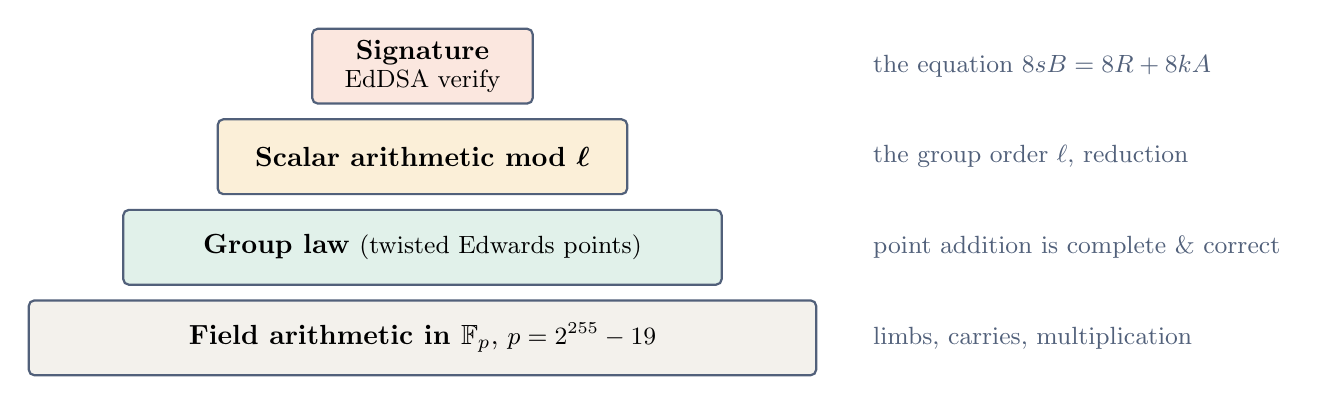
\begin{tikzpicture}[
  lay/.style={draw=ink2,thick,rounded corners=2pt,align=center,minimum height=0.95cm},
  note/.style={font=\small\color{ink2},align=left,anchor=west}
]
  \node[lay,fill=accentsoft,minimum width=2.8cm]  (sig) at (0,3.45) {\textbf{Signature}\\[-2pt]\small EdDSA verify};
  \node[lay,fill=warnsoft,minimum width=5.2cm]    (sca) at (0,2.3)  {\textbf{Scalar arithmetic mod $\boldsymbol{\ell}$}};
  \node[lay,fill=provensoft,minimum width=7.6cm]  (grp) at (0,1.15) {\textbf{Group law} \small (twisted Edwards points)};
  \node[lay,fill=codebg,minimum width=10cm]       (fld) at (0,0)    {\textbf{Field arithmetic in $\Fp$}, \small $p = 2^{255}-19$};
  \node[note] at (5.6,0)    {limbs, carries, multiplication};
  \node[note] at (5.6,1.15) {point addition is complete \& correct};
  \node[note] at (5.6,2.3)  {the group order $\ell$, reduction};
  \node[note] at (5.6,3.45) {the equation $8sB = 8R + 8kA$};
\end{tikzpicture}
\end{center}

By the end of this book you will be able to read --- and extend --- the real
proofs at every layer of this pyramid. The journey looks like this:

\begin{itemize}[leftmargin=1.4em]
\item \textbf{Chapters 2--5} teach Lean itself, from \code{\#eval 1+1} to
  proofs by induction and the automation that dispatches arithmetic goals.
\item \textbf{Chapters 6--7} build the mathematics: modular arithmetic, finite
  fields, and how to convince a paranoid kernel that a 77-digit number is
  prime.
\item \textbf{Chapters 8--9} cross the bridge from Rust to Lean: how real
  code is translated into a form we can reason about, and the single most
  important idea in the whole enterprise --- the \emph{denotation function}.
\item \textbf{Chapters 10--12} assemble the pyramid: field correctness, the
  ethics of axioms and honest boundaries, and the layers above.
\end{itemize}

\section{Proofs versus tests: the honest comparison}

Formal verification is not magic, and this book will never pretend otherwise.
It is worth being precise, right now, about what a machine-checked proof does
and does not give you.

\begin{center}
\begin{tabular}{@{}p{0.44\linewidth}p{0.48\linewidth}@{}}
\toprule
\textbf{Testing} & \textbf{Proving} \\
\midrule
Checks sampled inputs & Checks \emph{all} inputs \\
Cheap to start, cheap to run & Expensive to write, cheap to re-check \\
Finds bugs & Establishes their absence (w.r.t.\ the spec) \\
Trusts nothing & Trusts the spec, the model, the kernel \\
Silent about \emph{why} code is right & The proof \emph{is} the why \\
\bottomrule
\end{tabular}
\end{center}

That word \emph{spec} in the right column is the fine print, and it matters
enormously. A proof shows that code satisfies a specification. If the
specification says the wrong thing --- or says nothing, or is accidentally
trivial --- the proof is worthless no matter how green the checkmark. A
recurring theme of this book (it gets its own chapter,
Chapter~\ref{ch:honesty}) is how to read a verification claim skeptically:
What exactly was proven? Against which model of the code? Resting on which
axioms?

\begin{aha}
The most dangerous artifact in formal methods is not a wrong proof --- the
kernel prevents those. It is a \emph{correct proof of the wrong statement}.
Learning to smell those is as important as learning to write proofs at all.
\end{aha}

\section{Why Lean, and why now}

Twenty years ago, verifying real cryptographic C or Rust code was a heroic,
multi-year effort. Three things changed:

\begin{enumerate}[leftmargin=1.6em]
\item \textbf{Proof assistants matured.} Lean~4 is fast, pleasant, and comes
  with \emph{Mathlib}, a library of over a million lines of formalized
  mathematics --- finite fields and elliptic-curve ingredients included, so we
  do not start from bare axioms.
\item \textbf{Translation pipelines appeared.} Tools like \emph{Charon} and
  \emph{Aeneas} mechanically translate real Rust code into Lean definitions,
  so the thing we verify is derived from the code that ships, not a
  hand-transcribed approximation (Chapter~\ref{ch:rust}).
\item \textbf{Automation got serious.} Decision procedures like \lean{omega}
  (linear integer arithmetic) and \lean{decide} discharge the boring 90\% of
  goals, leaving humans the interesting 10\%.
\end{enumerate}

None of this made verification \emph{easy}. It made verification
\emph{possible for a well-prepared person in finite time} --- and preparing
you is exactly what this book is for.

\begin{tryit}
You do not need anything installed yet, but if you want to run code from
Chapter~2 onward, install Lean now. One command:
\begin{lstlisting}
curl https://elan.lean-lang.org/elan-init.sh -sSf | sh
\end{lstlisting}
Then open the \code{exercises/} folder of this repository in VS~Code with the
\emph{Lean 4} extension. The orange progress bar you will see is the proof
checker working through the file --- your new collaborator saying hello.
\end{tryit}

\section*{Exercises}

\exercise{A function takes two 255-bit inputs and is buggy on exactly one
input pair. Assume you can test $10^{9}$ random pairs per second. Estimate the
expected time to find the bug by random testing, in multiples of the age of
the universe ($\approx 4\times10^{17}$ seconds). You may approximate freely;
the point is the order of magnitude.}

\exercise{Give an example, from your own programming experience, of a bug that
survived a test suite. What property would a specification have needed to
state in order to exclude it?}

\exercise{(Discussion) A colleague says: ``Our crypto library is audited by
three firms every year; formal verification is redundant.'' Name one class of
defect audits are better at than proofs, and one class where proofs are
strictly stronger.}

\begin{checkpoint}
Before moving on, you should be able to explain to a friend:
(1) why testing fundamentally cannot establish correctness of a 255-bit
arithmetic function; (2) what a proof assistant's kernel is and why its small
size matters; (3) what a proof of correctness actually promises --- and the
role the specification plays in that promise.
\end{checkpoint}

\chapter{Meet Lean: A Language Where Programs and Proofs Live Together}
\label{ch:lean}

\section{First contact}

Lean~4 is two things wearing one syntax: a programming language (fast,
functional, compiled) and a proof assistant. You will learn both faces, but we
start with the friendlier one. Open a new file \code{Scratch.lean} and type:

\begin{lstlisting}[language=Lean]
#eval 1 + 1          -- 2
#eval 2 ^ 255 - 19   -- a 77-digit number, instantly
#eval "hello".length -- 5
\end{lstlisting}

\lean{\#eval} runs an expression and prints the result right in your editor.
Notice the second line: Lean's natural numbers are \emph{arbitrary precision}
by default. The number $2^{255}-19$ --- which will follow us through the whole
book --- is a perfectly ordinary value here, not an overflow.

\lean{\#check} asks a different question: not ``what is the value?'' but
``what is the \emph{type}?''

\begin{lstlisting}[language=Lean]
#check 1 + 1        -- 1 + 1 : Nat
#check "hello"      -- "hello" : String
#check (1 : Int) - 5 -- Int
\end{lstlisting}

\begin{bigidea}
In Lean, \textbf{every expression has a type}, and the type checker verifies
every file before anything runs. This obsession with types is not
bureaucracy --- in Chapter~\ref{ch:pat} it will turn out to be the entire
mechanism by which proofs work. Learn to read \code{e : T} as ``$e$ is of
type $T$'' --- or, with a squint we will justify later, ``$e$ is
\emph{evidence} for $T$.''
\end{bigidea}

\section{Definitions and functions}

New names are introduced with \lean{def}:

\begin{lstlisting}[language=Lean]
def p : Nat := 2 ^ 255 - 19

def double (n : Nat) : Nat := 2 * n

def isEven (n : Nat) : Bool := n % 2 == 0

#eval double 21      -- 42
#eval isEven p       -- false (p is odd, good: p is supposed to be prime!)
\end{lstlisting}

Three things to absorb from this snippet:

\begin{itemize}[leftmargin=1.4em]
\item Function application is written with a space: \lean{double 21}, not
  \code{double(21)}. It looks strange for a week and then all other syntax
  looks noisy forever after.
\item Every definition states its types: \lean{double} takes a \lean{Nat} and
  returns a \lean{Nat}. Lean can often infer types, but in this book we write
  them --- specifications are the whole game, and a type is a tiny
  specification.
\item Definitions are \emph{immutable equations}, not instructions. There is
  no ``assignment.'' \lean{p} \emph{is} $2^{255}-19$, forever.
\end{itemize}

Functions of several arguments simply take them in sequence, and functions
are values you can pass around:

\begin{lstlisting}[language=Lean]
def addMul (a b c : Nat) : Nat := a + b * c

def twice (f : Nat -> Nat) (x : Nat) : Nat := f (f x)

#eval twice double 10   -- 40
\end{lstlisting}

The type of \lean{twice} is worth staring at:
\lean{(Nat -> Nat) -> Nat -> Nat}. Arrows associate to the right, and a
multi-argument function is really a chain of single-argument ones --- this is
called \emph{currying}. Nothing about it needs memorizing now; it will become
muscle memory.

\section{Inductive types: building data from nothing}

Where do types like \lean{Nat} and \lean{Bool} come from? They are not
built-in magic. They are \emph{inductive types} --- data types defined by
listing every way to construct a value. Here is \lean{Bool}, exactly as the
core library defines it:

\begin{lstlisting}[language=Lean]
inductive Bool where
  | false : Bool
  | true  : Bool
\end{lstlisting}

Read: ``a \lean{Bool} is either \lean{false} or \lean{true}, and there is no
other way to make one.'' That closed-world clause is what makes case analysis
--- and later, proofs by cases --- airtight.

Now the star of the show. The natural numbers, following Peano's 1889 idea:

\begin{lstlisting}[language=Lean]
inductive Nat where
  | zero : Nat              -- 0 exists
  | succ (n : Nat) : Nat    -- every number has a successor
\end{lstlisting}

Every natural number is \lean{zero} wrapped in finitely many \lean{succ}s:
the number 3 \emph{is} \lean{succ (succ (succ zero))}. (Lean stores big
numbers efficiently under the hood, but \emph{reasons} about them through
this two-case skeleton.) Functions on inductive types are defined by
\emph{pattern matching} --- one equation per constructor:

\begin{lstlisting}[language=Lean]
def add : Nat -> Nat -> Nat
  | m, Nat.zero   => m
  | m, Nat.succ n => Nat.succ (add m n)
\end{lstlisting}

\begin{aha}
Look at what just happened. Addition --- the operation at the bottom of every
cryptosystem in this book --- is not an axiom or a CPU instruction here. It is
a \emph{two-line recursive program}, and every arithmetic fact we will ever
prove unwinds, ultimately, to these two equations. When Lean later claims
$a + b = b + a$ for \emph{all} numbers, it will be because the structure of
this definition forces it, not because anyone tested it.
\end{aha}

\begin{pitfall}
\lean{Nat} subtraction \emph{truncates}: \lean{\#eval (3 - 5 : Nat)} prints
\lean{0}, not $-2$, because natural numbers have nowhere to go below zero.
This single fact causes a large fraction of all beginner proof failures ---
an identity like $a - b + b = a$ is simply \emph{false} for \lean{Nat}. When
subtraction must mean subtraction, use \lean{Int}, or carry a hypothesis
$b \le a$. Real verification projects hit this constantly: machine arithmetic
wraps, truncates, and overflows, and the proofs must say so honestly.
\end{pitfall}

\section{Structures: records with guarantees}

The last data-building tool we need bundles several fields together:

\begin{lstlisting}[language=Lean]
structure Point where
  x : Int
  y : Int

def origin : Point := { x := 0, y := 0 }

#eval origin.x   -- 0
\end{lstlisting}

A preview of why this matters to us: the Rust type
\rust{struct FieldElement51(pub [u64; 5])} --- five 64-bit limbs representing
one element of $\Fp$ --- will arrive in Lean (Chapter~\ref{ch:rust}) as
essentially a structure holding an array of five machine words. The
verification question of this entire book is: \emph{do operations on those
five words faithfully implement arithmetic in $\Fp$?} Structures are how the
data crosses the bridge.

\section{Namespaces, Mathlib, and reading error messages}

Real developments organize names in \lean{namespace} blocks
(\lean{Nat.add}, \lean{Point.x}) and import the mathematical library:

\begin{lstlisting}[language=Lean]
import Mathlib
open Nat

#check Nat.Prime          -- the primality predicate, ready-made
#check ZMod               -- integers mod n -- our Chapter 6 home
\end{lstlisting}

And a word of comfort about \emph{error messages}. You will see many. Lean's
are precise and honest, and the single most useful habit you can develop this
week is: \textbf{read the expected/actual types in the message, slowly}. A
message like

\begin{lstlisting}
type mismatch: argument has type Int but is expected to have type Nat
\end{lstlisting}

is not the compiler being difficult; it is a specification violation caught at
the cheapest possible moment. Verification is this same experience scaled up:
the machine holds the line, and the line is exactly where you drew it.

\begin{tryit}
Open \code{exercises/Ch02.lean}. It contains the definitions from this chapter
with a few holes marked \lean{sorry} (a placeholder Lean accepts with a loud
warning). Replace each with a working definition and watch the warnings
disappear. In particular: define \lean{mul : Nat -> Nat -> Nat} by recursion,
using \lean{add} --- the same bootstrapping order (add, then mul) the real
field proofs follow.
\end{tryit}

\section*{Exercises}

\exercise{Define \lean{pow : Nat -> Nat -> Nat} (by recursion on the
exponent) and check with \lean{\#eval} that \lean{pow 2 10 = 1024}.}

\exercise{Define \lean{fib : Nat -> Nat}. Then evaluate \lean{fib 32}. Notice
the pause --- naive recursion is exponential. (Lean's \lean{\#eval} is fast;
your algorithm is slow. The distinction matters when we later care about
\emph{what} is being computed versus \emph{how}.)}

\exercise{Write a structure \lean{Rational} with fields \lean{num : Int} and
\lean{den : Nat}, and a function \lean{Rational.add}. What property of
\lean{den} can your type \emph{not} enforce yet? (Keep your answer; Chapter~3
gives you the tool to fix it.)}

\begin{checkpoint}
You should now be able to: evaluate and type-check expressions with
\lean{\#eval}/\lean{\#check}; define functions, including recursive ones over
\lean{Nat}; explain what an inductive type is and recite the two constructors
of \lean{Nat}; and state from memory what \lean{Nat} subtraction does on
$3 - 5$, and why that will matter.
\end{checkpoint}

\chapter{Propositions as Types: The Idea That Makes It All Work}
\label{ch:pat}

\section{A suspicious similarity}

Here are two things that look unrelated. First, a function that converts a
pair into something else:

\begin{lstlisting}[language=Lean]
def swap (pair : A x B) : B x A := (pair.2, pair.1)
\end{lstlisting}

Second, a fact of logic: \emph{if $A$ and $B$ both hold, then $B$ and $A$ both
hold.} To prove it, you would say: ``suppose I have evidence for $A$ and
evidence for $B$; then I can produce evidence for $B$ and evidence for $A$ ---
just present the same two pieces in the other order.''

That prose proof and that program are the \emph{same object}. The function
takes a pair of values and reorders it; the proof takes a pair of pieces of
evidence and reorders it. This is not an analogy or a teaching trick. It is a
theorem about logic and computation, discovered independently by logicians
(Curry, Howard) and now the load-bearing wall of Lean:

\begin{bigidea}
\textbf{The Curry--Howard correspondence.} A proposition can be read as a
type --- the type of its proofs. A proof is then simply a \emph{program} of
that type. Checking a proof is type-checking a program. There is no separate
``proof checker'' bolted onto Lean: the type checker you met in
Chapter~\ref{ch:lean} \emph{is} the proof checker.
\begin{center}
\begin{tabular}{@{}lll@{}}
\toprule
\textbf{Logic} & \textbf{Programming} & \textbf{In Lean} \\
\midrule
proposition $P$        & type            & \lean{P : Prop} \\
proof of $P$           & value/program of that type & \lean{h : P} \\
$P \to Q$ (implication)& function type   & \lean{P -> Q} \\
$P \land Q$ (and)      & pair type       & \lean{P /\ Q} \\
$P \lor Q$ (or)        & tagged union    & \lean{P \/ Q} \\
$\lnot P$ (not)        & \lean{P -> False} & \lean{Not P} \\
``true''               & type with one trivial value & \lean{True} \\
``false''              & \emph{empty} type & \lean{False} \\
\bottomrule
\end{tabular}
\end{center}
\end{bigidea}

Take a minute with the last row: \lean{False} is a type with \emph{no
constructors} --- no way to build a value. To prove a false statement you
would have to produce an inhabitant of an empty type. That is why the system
is sound: lies have no evidence, so lies do not type-check.

\section{Proofs are programs: first proofs}

Let us write actual proofs as actual programs. Implication is a function
type, so proving ``$P$ implies $P$'' means writing the identity function:

\begin{lstlisting}[language=Lean]
theorem p_implies_p (P : Prop) : P -> P :=
  fun h => h
\end{lstlisting}

Read \lean{fun h => h} aloud as a proof: ``assume $P$ holds --- call the
evidence $h$; then $P$ holds, by $h$.'' Every classical proof-writing phrase
has a program shape:

\begin{center}
\begin{tabular}{@{}ll@{}}
\toprule
\textbf{You say in prose} & \textbf{You write in Lean} \\
\midrule
``Assume $P$; call it $h$''       & \lean{fun h => ...} \\
``By hypothesis $h$''             & \lean{h} \\
``Apply lemma $f$ to fact $h$''   & \lean{f h} \\
``Both parts hold: ... and ...''  & \lean{And.intro pf1 pf2} \\
``From $h : P \land Q$, the first part'' & \lean{h.1} \\
\bottomrule
\end{tabular}
\end{center}

The pair-swapping example, now as an official theorem:

\begin{lstlisting}[language=Lean]
theorem and_swap (P Q : Prop) : P /\ Q -> Q /\ P :=
  fun h => And.intro h.2 h.1
\end{lstlisting}

And transitivity of implication is exactly function composition:

\begin{lstlisting}[language=Lean]
theorem imp_trans (P Q R : Prop) : (P -> Q) -> (Q -> R) -> (P -> R) :=
  fun pq qr => fun p => qr (pq p)
\end{lstlisting}

\begin{worked}{type-checking a proof by hand --- being the kernel once}
When Lean accepts \lean{and_swap}, what does it actually \emph{do}? It
type-checks the term --- and you can replay that check on paper, which is
the single best way to make Curry--Howard stop feeling like a slogan. The
term is \lean{fun h => And.intro h.2 h.1}; the claimed type is
\lean{P ∧ Q → Q ∧ P}. A type-checker works by walking the term and
maintaining a \emph{context} of what each variable is assumed to be ---
write the context on the left of a $\vdash$, the judgment on the right:
\[
\begin{array}{ll}
\text{1.} & \text{Goal: } \vdash \mathtt{fun\ h} \Rightarrow \dots \;:\; P \wedge Q \to Q \wedge P\\[2pt]
\text{2.} & \text{A \lean{fun} against an arrow type: put the argument in
             the context.}\\
          & h : P \wedge Q \;\vdash\; \mathtt{And.intro}\ h.2\ h.1 \;:\; Q \wedge P\\[2pt]
\text{3.} & \text{\lean{And.intro} needs a proof of } Q \text{ and a proof of } P
            \text{ (in that order, to build } Q \wedge P\text{).}\\[2pt]
\text{4.} & h : P \wedge Q \;\vdash\; h.2 : Q \qquad\text{✓ (second component
            of a conjunction)}\\
\text{5.} & h : P \wedge Q \;\vdash\; h.1 : P \qquad\text{✓ (first component)}\\[2pt]
\text{6.} & \text{All leaves check; the term has the claimed type. QED.}
\end{array}
\]
Every step is a bookkeeping rule --- ``\lean{fun} eats an arrow,''
``application must match the function's argument type,'' ``\lean{.1}
projects a pair.'' No inspiration occurred anywhere, which is the entire
point: \emph{checking} a proof is mechanical (a few thousand lines of
kernel), while \emph{finding} it is the creative act. Now deliberately
break it: try to check \lean{fun h => And.intro h.1 h.2} against the same
type. Step 4 demands $h.1 : Q$, but the context gives $h.1 : P$ ---
mismatch, rejected. A wrong proof does not check; you have just watched
soundness happen at the level where it lives.
\end{worked}

\begin{aha}
If you have ever composed two functions, you have already done everything
this proof does. The intimidating part of formal logic --- ``natural
deduction,'' ``inference rules'' --- turns out to be the part you knew from
programming all along. What logicians call \emph{modus ponens}, you call
\emph{calling a function}.
\end{aha}

\section{Equality and the proof that \texorpdfstring{$1+1=2$}{1+1=2}}

The proposition $a = b$ is also a type. Its only constructor is reflexivity
--- \lean{rfl} --- which proves \lean{a = a}. How can that ever prove
anything interesting? Because Lean \emph{computes} before comparing:

\begin{lstlisting}[language=Lean]
theorem one_plus_one : 1 + 1 = 2 := rfl
\end{lstlisting}

Lean unfolds \lean{1 + 1} using the two-line definition of addition from
Chapter~\ref{ch:lean}, arrives at \lean{2}, and sees that both sides are
\emph{literally the same value}. The equation holds by computation. This
mechanism --- \emph{definitional equality} --- is the engine that lets proofs
lean on programs, and later lets us prove facts about extracted Rust code by,
in part, just running it symbolically.

\begin{worked}{watching \lean{rfl} compute --- and watching it get stuck}
Both halves of the \lean{rfl} story fit on one sheet of paper, using the
\lean{add} equations from Chapter~\ref{ch:lean} (recursion on the second
argument; $s$ for successor). First, the success. To check
\lean{1 + 1 = 2}, the kernel normalizes both sides:
\[
1 + 1 \;=\; \mathtt{add}\ s(z)\ s(z)
\;=\; s(\mathtt{add}\ s(z)\ z)
\;=\; s(s(z))
\;=\; 2 .
\]
Two rewrite steps, both forced by the definition, and the two sides become
\emph{the same term} --- \lean{rfl} applies. Nothing about this argument
used the smallness of $1$: for \lean{2\textasciicircum{}255 - 19} the same normalization
runs on the efficient binary representation and succeeds just as surely
(only your patience is finite, not the principle).

Now the failure, on the same sheet. To check \lean{0 + n = n} for a
\emph{variable} $n$, the kernel again tries to normalize the left side:
\[
\mathtt{add}\ z\ n \;=\; ?
\]
Which defining equation applies? The first needs the second argument to be
$z$; the second needs it to be $s(\cdot)$. But $n$ is \emph{opaque} --- an
arbitrary variable exhibits neither constructor. No equation fires, the
term is stuck, the two sides stay different terms, \lean{rfl} fails. Note
precisely what failed: not the \emph{truth} of the statement (it is true
for every concrete $n$, and each instance --- \lean{0 + 5 = 5}, say ---
normalizes fine), but computation's ability to see it \emph{uniformly}.
Whenever a variable blocks the recursion pattern, computation ends and
\emph{induction} must take over --- now you can predict, before trying,
which equalities are \lean{rfl}s. Test yourself: \lean{n + 0 = n}?
(Second argument is the concrete $z$ --- first equation fires ---
\lean{rfl}.) \lean{n * 1 = n}? Depends on which argument \lean{mul}
recurses on; go read your Chapter~\ref{ch:lean} solution and decide.
\end{worked}

\begin{pitfall}
\lean{rfl} proves $2^{255} - 19$-sized computations happily, but it can only
prove what computation alone can see. \lean{n + 0 = n} is \lean{rfl} (the
definition's first equation matches), yet \lean{0 + n = n} is \emph{not} ---
recursion is on the \emph{second} argument, and \lean{n} is an opaque
variable, so nothing unfolds. The statement is still true; it just needs a
real proof (induction --- next chapter). The asymmetry feels unfair for about
a day. Then it becomes your sharpest mental model of what a computer can and
cannot know for free.
\end{pitfall}

\section{Universals, existentials, and dependent types}

Cryptographic specifications are universal statements: ``\emph{for all}
inputs, the output is correct.'' In Lean, $\forall$ is a function type whose
\emph{result type mentions the argument}:

\begin{lstlisting}[language=Lean]
theorem add_self_even : forall n : Nat, isEven (n + n) = true := ...
\end{lstlisting}

A proof of \lean{forall n, P n} is a function that eats any \lean{n} and
returns a proof of \lean{P n} --- one uniform recipe covering all the
infinitely many cases at once. This is precisely the thing testing could not
give us in Chapter~\ref{ch:why}: testing produces finitely many
\lean{P 3, P 17, P 42}; a proof produces the function.

\begin{worked}{a universal statement as one uniform recipe}
Feel the difference between testing and proving on the smallest
interesting universal: \emph{every number of the form $n + n$ is even},
where $\mathrm{even}(m) := \exists k,\, m = 2k$. The testing mind
samples: $3 + 3 = 6 = 2\cdot 3$ ✓, $7 + 7 = 14 = 2 \cdot 7$ ✓, and after
a while believes. The proving mind writes \emph{one function}:
\[
\text{given any } n, \text{ return the witness } k := n
\text{ together with the fact } n + n = 2n .
\]
That is the entire proof --- a recipe that, \emph{handed any} $n$,
produces the evidence for \emph{that} $n$: for $n = 3$ it yields witness
$3$ and the equation $6 = 6$; for $n = 2^{254}$ it yields witness
$2^{254}$ just as cheaply, because the recipe never looks at the digits.
In Lean:
\begin{lstlisting}[language=Lean]
theorem add_self_even : ∀ n : Nat, ∃ k, n + n = 2 * k :=
  fun n => ⟨n, (Nat.two_mul n).symm⟩
\end{lstlisting}
Read the term against the table: \lean{fun n =>} consumes the $\forall$
(a function, as promised); \lean{⟨n, ...⟩} produces the $\exists$ (a
witness paired with evidence). Now the punchline for this book: every
correctness certificate in the companion repositories has exactly this
shape --- \lean{∀ a b, Bnd a → Bnd b → ∃ c, ...} --- a function that
eats \emph{arbitrary} 255-bit inputs and manufactures the evidence for
them. When Chapter~\ref{ch:why} said proofs cover $10^{153}$ input pairs
at once, this recipe-not-samples mechanism is \emph{how}. No induction
was even needed here; when the recipe does need to consult the
structure of $n$, induction (Chapter~\ref{ch:tactics}) is how a recipe
consults structure.
\end{worked}

Dually, \lean{exists n, P n} is proved by handing over a concrete witness
together with evidence: \lean{Exists.intro 4 pf}. And remember the
\lean{Rational} exercise from last chapter --- the denominator you could not
keep nonzero? Dependent types fix it by letting data carry proofs:

\begin{lstlisting}[language=Lean]
structure Rational where
  num   : Int
  den   : Nat
  den_ne_zero : den ≠ 0    -- a PROOF, stored inside the value
\end{lstlisting}

No value of this type with a zero denominator can ever be constructed,
anywhere, by anyone. In the real Ed25519 development this exact pattern
appears as a \emph{bounds invariant}: a field element travels together with
the proof that its five limbs are small enough not to overflow the next
multiplication. The data structure makes the unsafe states unrepresentable.

\section{What about proof by contradiction?}

One more resident of the logical zoo. Lean's core logic is
\emph{constructive}: a proof of existence builds a witness. Classical
reasoning --- ``it's either true or false, and not false, hence true'' --- is
available the moment you want it (Mathlib imports it as \lean{Classical.choice},
and we will meet it again on the trust ledger in Chapter~\ref{ch:honesty}),
but it is an \emph{ingredient you can see}, not smuggled seasoning. When a
verification result says ``this proof uses only \lean{propext},
\lean{Classical.choice}, \lean{Quot.sound},'' that is a complete list of the
logical beliefs you are being asked to hold. Three. You can audit them over
coffee.

\begin{tryit}
Open \code{exercises/Ch03.lean} and prove, as programs (no tactics yet!):
\lean{P -> Q -> P}; \ \lean{(P /\ Q) -> (P \/ Q)}; \ and modus ponens
\lean{P -> (P -> Q) -> Q}. Each is a one-liner. Feel free to be delighted
when the pieces click together like typed Lego.
\end{tryit}

\section*{Exercises}

\exercise{Prove \lean{and_assoc : (P /\ Q) /\ R -> P /\ (Q /\ R)} as a
term-mode program using \lean{h.1}, \lean{h.2}, and \lean{And.intro}.}

\exercise{Prove \lean{or_swap : P \/ Q -> Q \/ P}. You will need case
analysis on which side holds: \lean{match h with | Or.inl p => ... | Or.inr q => ...}}

\exercise{\lean{Not P} is \emph{defined} as \lean{P -> False}. Using only
that, prove \lean{P -> Not (Not P)}. Write down in one sentence what program
you just wrote.}

\exercise{(Thought) Explain to a skeptical friend why a type with no
constructors is the right representation of falsehood --- and what would go
wrong with the whole edifice if someone added a constructor to it.}

\section*{Solutions and pathways}
\solutionsintro

\solhead{3.1}
\pathway Draw the shapes before writing the term. You \emph{have} a
nested pair $((p,q),r)$; you \emph{owe} $(p,(q,r))$. The projections
\lean{.1}/\lean{.2} take pairs apart; \lean{And.intro} puts them together;
the whole proof is re-parenthesizing a package. Chase each component: where
does $p$ live inside the input? At \lean{h.1.1}.
\answer
\begin{lstlisting}[language=Lean]
theorem and_assoc' : (P ∧ Q) ∧ R → P ∧ (Q ∧ R) :=
  fun h => And.intro h.1.1 (And.intro h.1.2 h.2)
\end{lstlisting}
Read it back as prose: ``from $((p,q),r)$, produce $(p,(q,r))$.'' If your
version has the components in a different arrangement, type-check it by
hand as in the worked example --- exactly one arrangement survives step 4.

\solhead{3.2}
\pathway A disjunction is a \emph{tagged} value --- you cannot project both
sides out of it (only one exists!), so the projection style of 3.1 is
unavailable. The only way to consume \lean{P ∨ Q} is case analysis: handle
each tag. In term mode that is a \lean{match} with two arms; each arm
holds evidence for one side and must rebuild the output disjunction with
the \emph{other} tag.
\answer
\begin{lstlisting}[language=Lean]
theorem or_swap : P ∨ Q → Q ∨ P :=
  fun h => match h with
    | Or.inl p => Or.inr p
    | Or.inr q => Or.inl q
\end{lstlisting}
Note the tag flip: evidence that arrived tagged ``left'' leaves tagged
``right'' and vice versa. The compiler checks \emph{exhaustiveness} ---
delete an arm and the proof is rejected, because a case of reality would
be unhandled. Compare with \lean{and_swap}: same theorem shape, entirely
different evidence plumbing. The connective dictates the program.

\solhead{3.3}
\pathway Unfold the abbreviation twice.
$\lnot P = P \to \mathtt{False}$, so
$\lnot\lnot P = (P \to \mathtt{False}) \to \mathtt{False}$. The goal
$P \to \lnot\lnot P$ is therefore
$P \to (P \to \mathtt{False}) \to \mathtt{False}$: two arguments --- a
proof and a refuter --- and you must produce \lean{False}. There is exactly
one way to get a \lean{False}: apply the refuter.
\answer
\begin{lstlisting}[language=Lean]
theorem not_not_intro : P → ¬¬P :=
  fun p f => f p
\end{lstlisting}
The one-sentence description: \emph{``given evidence $p$ and any would-be
refutation $f$ of $P$, feed $p$ to $f$ --- the refutation defeats
itself.''} It is modus ponens wearing a philosophy costume. (The converse,
$\lnot\lnot P \to P$, is \emph{not} writable in this plain style --- you
would have to conjure a $p$ out of a function that only consumes them.
That is the constructive/classical boundary of the last section, met in
the wild.)

\solhead{3.4}
\pathway Recall what a proof of \lean{False} would be --- a value of the
empty type --- and follow the consequences of the type not being empty
anymore.
\answer (Model answer.) ``Falsehood must be the proposition with \emph{no
evidence}: if you could construct a proof of \lean{False}, `proof' would
stop meaning anything. In this system that is not a moral claim but a
structural one --- \lean{False} is an inductive type with zero
constructors, so no closed term of that type exists. Every other
proposition's strength derives from this emptiness: $\lnot P$ means
$P \to \mathtt{False}$, and the principle `from \lean{False}, anything'
is safe precisely because its premise is unreachable. Add one constructor
\lean{oops : False} and watch the edifice fall: \lean{False.elim oops}
now proves \emph{every} proposition --- $1 = 2$, `this code is correct,'
everything --- and every certificate ever checked becomes worthless
simultaneously. The kernel's whole job is to be the thing that never lets
\lean{oops} in.'' Connect this forward: Chapter~\ref{ch:honesty}'s
\lean{\#print axioms} audit is, at bottom, checking that nobody smuggled
in an \lean{oops} dressed as an axiom.

\begin{checkpoint}
You should now be able to: translate each logical connective into its type
($\to$, $\land$, $\lor$, $\lnot$, $\forall$, $\exists$); write small proofs
as terms; explain why \lean{rfl} proves \lean{1 + 1 = 2} but not
\lean{0 + n = n}; and articulate the Curry--Howard slogan --- \emph{proofs
are programs, propositions are types, checking is type-checking} --- with a
straight face and genuine conviction.
\end{checkpoint}

\chapter{Tactics: Proving as a Dialogue}
\label{ch:tactics}

\section{From programs to conversations}

Writing proofs as raw programs, as in Chapter~\ref{ch:pat}, is honest work,
but it scales badly: a real correctness proof for field multiplication would
be a program the size of a small compiler. Nobody writes those by hand.
Instead, Lean offers \emph{tactic mode}: an interactive dialogue where you
issue commands and Lean builds the proof program for you, step by step,
showing you the remaining work after each move.

You enter the dialogue with the keyword \lean{by}:

\begin{lstlisting}[language=Lean]
theorem and_swap (P Q : Prop) : P ∧ Q → Q ∧ P := by
  intro h
  constructor
  · exact h.2
  · exact h.1
\end{lstlisting}

Place your cursor after \lean{by} in the editor and Lean shows the
\textbf{goal state} --- the exact logical situation at that point:

\begin{lstlisting}
P Q : Prop
⊢ P ∧ Q → Q ∧ P
\end{lstlisting}

Everything above the turnstile \(\vdash\) is what you \emph{have} (the
context); the line after it is what you \emph{owe} (the goal). Every tactic
transforms this picture. After \lean{intro h}, the hypothesis moves above the
line; after \lean{constructor}, the goal splits in two. Proving becomes a
game whose board you can always see.

\begin{bigidea}
A tactic proof is a \textbf{recorded conversation with the goal state}. The
skill of proving is not memorizing tactic names --- it is learning to
\emph{read the goal state} and recognize which of a handful of moves makes it
simpler. Below is the core vocabulary; it covers the vast majority of every
proof in the real Ed25519 development.
\end{bigidea}

\begin{center}
\begin{tabular}{@{}lll@{}}
\toprule
\textbf{Tactic} & \textbf{When the goal looks like...} & \textbf{Effect} \\
\midrule
\lean{intro h}   & \lean{P → Q}, \ \lean{∀ x, P x} & assume it; name the evidence \\
\lean{exact e}   & anything      & finish: \lean{e} is a proof of the goal \\
\lean{apply f}   & \lean{Q}, given \lean{f : P → Q} & reduce the goal to \lean{P} \\
\lean{constructor} & \lean{P ∧ Q}, \lean{P ↔ Q}, ... & split into pieces \\
\lean{cases h}   & have \lean{h : P ∨ Q} (or \(\wedge\), \lean{∃}) & case analysis on \lean{h} \\
\lean{rw [eq]}   & contains a rewritable subterm & replace using equation \lean{eq} \\
\lean{simp}      & simplifiable clutter & rewrite with a lemma database \\
\lean{induction n} & \lean{∀ n : Nat, ...} & base case + inductive step \\
\lean{rfl}       & \lean{a = a} after computation & close by computation \\
\bottomrule
\end{tabular}
\end{center}

\section{Rewriting: equality as a tool}

The workhorse tactic of equational reasoning is \lean{rw} (rewrite). Given a
proven equation, it replaces one side by the other inside your goal:

\begin{lstlisting}[language=Lean]
example (a b : Nat) (h : a = b) : a + a = b + b := by
  rw [h]      -- goal becomes: b + b = b + b, closed by rfl automatically
\end{lstlisting}

Chains of rewrites read like the two-column proofs of school geometry,
except a machine checks every line. Here is commutativity-and-associativity
shuffling, Mathlib lemmas by name:

\begin{lstlisting}[language=Lean]
example (a b c : Nat) : a + b + c = c + b + a := by
  rw [Nat.add_comm a b]        -- b + a + c = c + b + a
  rw [Nat.add_assoc]           -- b + (a + c) = c + b + a
  rw [Nat.add_comm a c]        -- b + (c + a) = c + b + a
  rw [← Nat.add_assoc]         -- b + c + a = c + b + a
  rw [Nat.add_comm b c]        -- done
\end{lstlisting}

The arrow \(\leftarrow\) rewrites right-to-left. Nobody enjoys writing five-line
shuffles like this, which is exactly why Chapter~\ref{ch:automation}
introduces \lean{ring} --- but you must \emph{once} feel the manual version to
understand what the automation is doing on your behalf.

\section{Induction: the tactic that conquers infinity}

Remember the embarrassment of Chapter~\ref{ch:pat}: \lean{0 + n = n} does not
hold by computation. Now we can prove it --- by induction, the proof
technique that inductive types were born for:

\begin{lstlisting}[language=Lean]
theorem zero_add (n : Nat) : 0 + n = n := by
  induction n with
  | zero      => rfl                -- 0 + 0 = 0: computes
  | succ k ih => rw [Nat.add_succ, ih]
\end{lstlisting}

The \lean{induction} tactic converts a statement about \emph{all} naturals
into two finite obligations: the statement for \lean{zero}, and the statement
for \lean{succ k} \emph{assuming it for} \lean{k} (the induction hypothesis
\lean{ih}). Because every natural number is built from those two
constructors, the two cases cover infinity.

\begin{aha}
Induction is not a new axiom to swallow --- it falls out of the inductive
definition of \lean{Nat} itself. ``Every \lean{Nat} is \lean{zero} or a
\lean{succ}'' \emph{is} the license to do case analysis; recursion on the
structure \emph{is} the induction. Data and proof principle are two views of
the same declaration. This is Curry--Howard paying rent again.
\end{aha}

\begin{pitfall}
When a proof gets stuck, resist the urge to try random tactics --- the
formal-methods equivalent of mashing buttons. The goal state is telling you
something. Three honest questions unstick most situations: (1)~Is the
statement actually true as written --- check a small example with
\lean{\#eval}! (2)~Am I missing a hypothesis --- is there an unstated bound or
nonzero condition? (3)~Is my induction on the right variable? In the real
projects behind this book, ``the proof is stuck'' was, more often than not,
the \emph{statement} being subtly wrong --- a truncated subtraction, a missing
bound. The proof assistant was the messenger.
\end{pitfall}

\section{Structuring real proofs: \texttt{have} and \texttt{calc}}

Big proofs are not flat lists of tactics; they are structured arguments with
named intermediate results. The \lean{have} tactic states and proves a
stepping stone; \lean{calc} lays out a chain of equalities or inequalities
the way you would on a whiteboard:

\begin{lstlisting}[language=Lean]
example (a b : Nat) (h : a = 2 * b) : a + a = 4 * b := by
  have h2 : a + a = 2 * a := by rw [Nat.two_mul]
  calc a + a = 2 * a       := h2
       _     = 2 * (2 * b) := by rw [h]
       _     = 4 * b       := by rw [← Nat.mul_assoc]
\end{lstlisting}

This style is not cosmetic. In the verified field arithmetic you will read
later, a single multiplication correctness proof is a \lean{calc} chain
tracking limb products through carries --- dozens of steps, each trivial,
whose \emph{composition} is the theorem. \lean{have} and \lean{calc} are how
proofs stay readable at that scale; they are also how they stay
\emph{maintainable}, because a broken step localizes the damage to one line.

There is one more structuring fact worth knowing early, because it saved the
real project from a crash-course (literally --- see
Chapter~\ref{ch:honesty}): breaking a proof into small named \lean{have}
steps also controls the proof assistant's \emph{memory appetite}. A monolithic
``figure it all out at once'' tactic call over a huge context can consume
gigabytes; ten targeted steps, pennies each, prove the same thing. Structure
is not just style --- it is engineering.

\begin{tryit}
Open \code{exercises/Ch04.lean}. It sets up each theorem with the goal state
drawn in a comment, then asks you to: prove \lean{and_swap} in tactic mode;
prove \lean{zero_add} \emph{without} peeking above; and repair a broken
\lean{calc} chain in which exactly one step is wrong. The third
exercise is secretly the most realistic job training in this book.
\end{tryit}

\section*{Exercises}

\exercise{Prove by induction: \lean{∀ n : Nat, n + 0 = n} and
\lean{∀ n m : Nat, n + succ m = succ (n + m)}. (These are the mirror images
of the definitional equations --- the ones computation gives you for free ---
and together they yield commutativity.)}

\exercise{Using the previous exercise, prove
\lean{∀ n m : Nat, n + m = m + n} by induction on \lean{m}. Write out, in
one prose sentence per case, what each branch of your proof says.}

\exercise{Prove \lean{∀ n : Nat, 2 * n = n + n} twice: once with
\lean{induction}, once with a single \lean{rw} using a Mathlib lemma you find
yourself (search hint: \lean{exact?} asks Lean to search for you).}

\exercise{(Reading) In the goal state
\lean{h : a < 2\textasciicircum{}51 ⊢ a * 19 < 2\textasciicircum{}56}, no induction is needed --- this is pure
arithmetic. Which tactic from the table would you \emph{guess} handles it?
(Answer next chapter; your guess is the point.)}

\begin{checkpoint}
You should now be able to: read a goal state (context, turnstile, goal);
drive the core tactics \lean{intro}, \lean{exact}, \lean{apply},
\lean{cases}, \lean{rw}, \lean{induction}; structure a multi-step argument
with \lean{have} and \lean{calc}; and --- most importantly --- when stuck,
interrogate the \emph{statement} before blaming the proof.
\end{checkpoint}

\chapter{Numbers and Automation: Making the Machine Do the Boring Parts}
\label{ch:automation}

\section{The 90/10 rule of verification}

Here is a trade secret: most of a real verification effort is not clever.
Opening the correctness proof of Ed25519 field multiplication, you will find
that the overwhelming majority of proof obligations are statements like

\[
a < 2^{51} \;\wedge\; b < 2^{51} \;\Longrightarrow\; a + b < 2^{52},
\qquad\qquad
(a + b) \cdot c = a\cdot c + b\cdot c,
\]

--- bookkeeping a patient undergraduate could verify by hand in a minute
each. There are \emph{thousands} of them. The craft of modern verification is
to hand exactly this 90\% to decision procedures --- tactics that implement a
complete algorithm for a well-defined logical fragment --- and save the human
for the 10\% that needs insight. This chapter is your tour of the arsenal.

\section{\texttt{omega}: linear arithmetic, decided}

The tactic you will use more than any other in this book's domain is
\lean{omega}. It completely decides \emph{linear arithmetic} over integers
and naturals: any goal built from variables, constants, $+$, $-$,
multiplication \emph{by constants}, $=$, $<$, $\le$, $\lnot$, $\wedge$,
$\vee$, including the hypotheses in context.

\begin{lstlisting}[language=Lean]
example (a b : Nat) (h1 : a < 2^51) (h2 : b < 2^51) :
    a + b < 2^52 := by omega

example (a b : Nat) (h : a ≤ b) : a + (b - a) = b := by omega
  -- note: truncated Nat subtraction handled CORRECTLY -- omega knows
\end{lstlisting}

That second example deserves a salute: \lean{omega} understands \lean{Nat}
truncation natively, defusing the Chapter~\ref{ch:lean} pitfall by algorithm
rather than by vigilance. When the goal is false, \lean{omega} \emph{fails} ---
it is a decision procedure, so failure on a linear goal means the goal (with
the hypotheses in view) is simply not true. That property turns \lean{omega}
into a \emph{statement-debugging} tool: if it refuses your ``obviously true''
bound, go find the counterexample; there is one.

\begin{pitfall}
\lean{omega} does not touch multiplication of two \emph{variables}
($a \cdot b$ is not linear), division in general, or bit-shifts by variables.
For a goal mixing $a \cdot b$ with bounds, you often first name the product
--- \lean{have hab : a * b ≤ 2\textasciicircum{}102 := ...} using a multiplication
monotonicity lemma --- and then let \lean{omega} finish with \lean{hab} as an
opaque atom. This two-step, \emph{bound the nonlinear part, then release the
linear solver}, is the single most-used proof pattern in verified field
arithmetic. You will write it dozens of times, and by Chapter~\ref{ch:field}
it will feel like breathing.
\end{pitfall}

\section{\texttt{decide}: when truth is a computation}

Some propositions can be checked by running an algorithm to completion:
``$97$ is prime,'' ``these two sorted lists are equal,'' ``$x^3 = x$ for all
$x$ in $\Zmod{6}$'' (six cases --- check them all). For any such
\emph{decidable} proposition, the \lean{decide} tactic runs the decision
algorithm inside Lean's kernel and turns the answer into a proof:

\begin{lstlisting}[language=Lean]
example : Nat.Prime 97 := by decide
example : ∀ x : ZMod 6, x^3 = x^3 := by decide   -- finite: try all six
\end{lstlisting}

The magic and the limitation are the same fact: the \emph{kernel itself}
re-executes the computation. That makes \lean{decide} unimpeachable --- and
completely hopeless for our 77-digit prime $2^{255}-19$, where trial division
would outlast the universe. There is a variant, \lean{native_decide}, that
compiles the check to native code first --- fast enough! --- but it makes the
compiler part of your trusted base, an IOU we will scrutinize hard in
Chapters~\ref{ch:prime} and~\ref{ch:honesty}. For now, the rule of the house:
\textbf{\lean{decide} yes, \lean{native_decide} never in a final certificate.}

\section{\texttt{ring} and \texttt{norm\_num}: algebra on tap}

The five-line commutativity shuffle from Chapter~\ref{ch:tactics}? Here is
the grown-up version:

\begin{lstlisting}[language=Lean]
example (a b c : Nat) : a + b + c = c + b + a := by ring

example (a b : ZMod p) : (a + b)^2 = a^2 + 2*a*b + b^2 := by ring

example : (2:Int)^255 - 19 > 2^254 := by norm_num
\end{lstlisting}

\lean{ring} proves any identity that holds in every commutative ring ---
polynomial rearrangements, binomial expansions, distributivity avalanches ---
by normalizing both sides to a canonical polynomial form and comparing.
\lean{norm_num} evaluates concrete numeric facts, comfortable with numbers of
any size. Between \lean{omega}, \lean{ring}, and \lean{norm_num} you now hold
the three keys that open most arithmetic doors:

\begin{center}
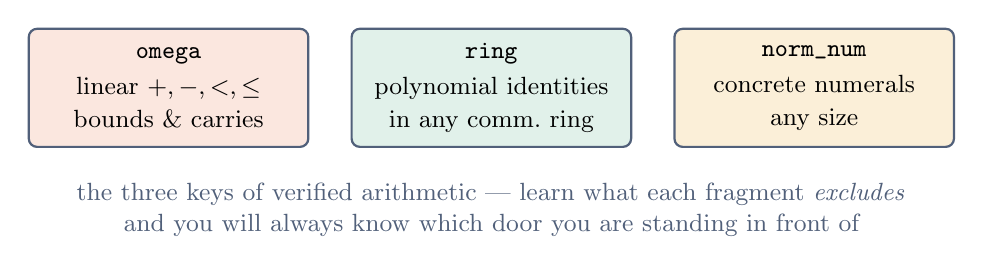
\begin{tikzpicture}[
  key/.style={draw=ink2,thick,rounded corners=3pt,fill=white,align=center,
              minimum width=3.55cm,minimum height=1.5cm},
]
  \node[key,fill=accentsoft] (o) at (0,0)
    {\textbf{\code{omega}}\\[1pt]\small linear $+,-,<,\le$\\\small bounds \& carries};
  \node[key,fill=provensoft] (r) at (4.1,0)
    {\textbf{\code{ring}}\\[1pt]\small polynomial identities\\\small in any comm.\ ring};
  \node[key,fill=warnsoft] (n) at (8.2,0)
    {\textbf{\code{norm\_num}}\\[1pt]\small concrete numerals\\\small any size};
  \node[font=\small\color{ink2},align=center] at (4.1,-1.55)
    {the three keys of verified arithmetic --- learn what each fragment
     \emph{excludes}\\ and you will always know which door you are standing in front of};
\end{tikzpicture}
\end{center}

\section{\texttt{simp}: the rewriting engine, and how to hold it}

\lean{simp} rewrites the goal to exhaustion using a curated database of
thousands of ``simplification'' lemmas ($x + 0 \rightsquigarrow x$,
\lean{List.length (a :: l)} $\rightsquigarrow$ \lean{l.length + 1}, ...). It
is the most powerful tactic in Lean and the easiest to misuse. Used well, it
clears brush so the real argument stands out. Used lazily ---
\lean{simp [*]} with every hypothesis thrown in, in a context of sixty
accumulated facts --- it becomes a search over an enormous rewrite space:
slow, fragile under library updates, and occasionally a memory monster.

This is not hypothetical. During the development this book accompanies, a
single over-broad \lean{simp}-style discharge in a fat context consumed
twelve gigabytes of RAM and took down the machine. The postmortem produced
house rules worth adopting from day one:

\begin{itemize}[leftmargin=1.4em]
\item Prefer \lean{simp only [lemma1, lemma2]} --- an explicit lemma list ---
  in anything you intend to keep.
\item Let \lean{simp?} tell you the list: run it once interactively, then
  paste the \lean{simp only [...]} it suggests into the file.
\item Keep contexts lean (pun intended): a proof with sixty hypotheses in
  scope wants to be five \lean{have}-steps with twelve each.
\end{itemize}

\begin{bigidea}
Automation is a \emph{contract}, not a slot machine. Each tactic decides a
known fragment: \lean{omega} linear arithmetic, \lean{ring} ring identities,
\lean{decide} finite computation, \lean{simp only} a rewrite system you
chose. The professional habit is to know \emph{which} contract you are
invoking --- then failure is information (``this goal is not linear''; ``this
identity needs the modulus''), never mystery.
\end{bigidea}

\begin{tryit}
Open \code{exercises/Ch05.lean}: ten arithmetic goals, each solvable by
exactly one of \lean{omega} / \lean{ring} / \lean{norm_num} / \lean{decide}.
Your task is not just to close them but to close each with the \emph{right}
tool --- the file rejects overkill by design. Goal number ten is the
Chapter~\ref{ch:tactics} cliffhanger:
\lean{a < 2\textasciicircum{}51 → a * 19 < 2\textasciicircum{}56}. (It is not linear --- $19$ is a constant, so
it is! Think, then fire.)
\end{tryit}

\section*{Exercises}

\exercise{For each, name the tactic and predict success before running:
(a) \lean{(a+b)*(a-b) = a*a - b*b} over \lean{Int};
(b) \lean{a < 100 → b < 100 → a*b < 10000} over \lean{Nat};
(c) \lean{Nat.Prime 65537};
(d) \lean{2\textasciicircum{}51 + 2\textasciicircum{}51 = 2\textasciicircum{}52}.}

\exercise{Goal (b) above is nonlinear, yet \lean{omega} alone fails while the
two-step pattern (bound the product with
\lean{Nat.mul_lt_mul} machinery, then \lean{omega}) succeeds. Carry it out.
Time yourself; the pattern should take under five minutes by the second
attempt.}

\exercise{Find a true statement about \lean{Nat} that \emph{no} tactic in
this chapter proves in one shot, and sketch in prose how you would decompose
it. (Anything genuinely inductive works --- automation here decides
arithmetic fragments, not all of mathematics.)}

\begin{checkpoint}
You should now be able to: match a goal to its decision procedure by the
shape of its operators; execute the bound-then-omega pattern for nonlinear
bounds; explain why \lean{decide} is trustworthy and where it hits its
computational wall; and state the \lean{simp} discipline --- and the story of
why this book is unusually sincere about it.
\end{checkpoint}

\chapter{Modular Arithmetic: The Number System Cryptography Lives In}
\label{ch:modular}

\section{Clock arithmetic, taken seriously}

You already compute modulo twelve every day: four hours after ten o'clock is
two o'clock. Wrap-around arithmetic --- add, overflow the dial, keep the
remainder --- is the entire idea of \emph{modular arithmetic}. Cryptography's
only twist is the size of the clock: Ed25519's dial has
\[
p = 2^{255} - 19
\]
hours on it --- a 77-digit prime. Everything else --- the wrap-around, the
remainder-taking, the algebra --- is the twelve-hour clock you already know.

Formally, we write $a \equiv b \pmod{n}$ when $n$ divides $a - b$, and we
collect all integers with the same remainder into one object: the world
$\Zmod{n}$ has exactly $n$ elements, $\{0, 1, \dots, n-1\}$, with addition
and multiplication that wrap. In Lean/Mathlib this world is a first-class
type, and computation in it is exactly what you would hope:

\begin{lstlisting}[language=Lean]
#eval (7 + 8 : ZMod 12)    -- 3     (fifteen o'clock is three o'clock)
#eval (5 * 9 : ZMod 12)    -- 9
#eval (3 - 7 : ZMod 12)    -- 8     (subtraction wraps -- no truncation!)

def p : Nat := 2^255 - 19
#eval (2^255 : ZMod p)     -- 19    (of course: 2^255 = p + 19)
\end{lstlisting}

Note the third line with relief: unlike \lean{Nat}, subtraction in
\lean{ZMod n} is a total, well-behaved inverse of addition. Every element has
a negative. In algebra terms, $\Zmod{n}$ is a \emph{commutative ring} --- and
Lean knows it, so the \lean{ring} tactic from Chapter~\ref{ch:automation}
works there natively.

\section{Division: where primes enter}

Rings give us $+$, $-$, $\times$. Cryptography also needs $\div$ --- and
division is where the modulus stops being a size parameter and starts being a
design decision. Dividing by $a$ means multiplying by some $a^{-1}$ with
$a \cdot a^{-1} = 1$. Does such an inverse exist? On the twelve-hour clock,
try to invert $4$: the multiples of $4$ are $4, 8, 0, 4, 8, 0, \dots$ ---
the value $1$ never appears. $4$ has no inverse mod $12$, because $4$ and
$12$ share the factor~$4$.

\begin{bigidea}
In $\Zmod{n}$, the element $a$ is invertible exactly when
$\gcd(a, n) = 1$. So if $n = p$ is \textbf{prime}, \emph{every} nonzero
element is invertible: you can divide freely, and $\Zmod{p}$ earns the title
of \textbf{field}, written $\Fp$. Fields are the arithmetic paradise where
linear algebra, polynomial factoring, and elliptic-curve geometry all work.
This --- and only this --- is why cryptographic moduli are prime: primality
is the entry ticket to division.
\end{bigidea}

\begin{center}
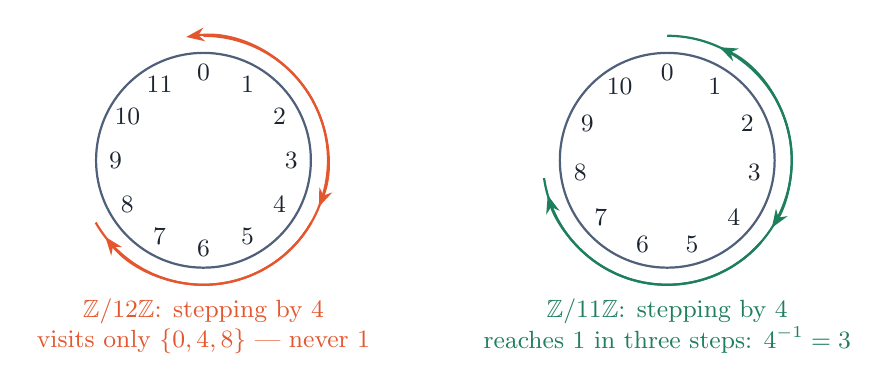
\begin{tikzpicture}[scale=0.62,every node/.style={font=\small}]
  % Z/12 clock: multiples of 4 stuck in a cycle
  \begin{scope}
    \draw[ink2,thick] (0,0) circle (2.2);
    \foreach \i in {0,...,11} \node[color=ink] at ({90-\i*30}:1.8) {\i};
    \foreach \s/\t in {0/4, 4/8, 8/0}
      \draw[-{Stealth},accent,thick] ({90-\s*30}:2.55) arc ({90-\s*30}:{90-\t*30+8}:2.55);
    \node[color=accent,align=center] at (0,-3.4) {$\Zmod{12}$: stepping by $4$\\ visits only $\{0,4,8\}$ --- never $1$};
  \end{scope}
  % Z/11 clock: multiples of 4 reach 1
  \begin{scope}[xshift=9.5cm]
    \draw[ink2,thick] (0,0) circle (2.2);
    \foreach \i in {0,...,10} \node[color=ink] at ({90-\i*32.72}:1.8) {\i};
    \foreach \s/\t in {0/4, 4/8, 8/1}
      \draw[-{Stealth},proven,thick] ({90-\s*32.72}:2.55) arc ({90-\s*32.72}:{90-\t*32.72+8}:2.55);
    \node[color=proven,align=center] at (0,-3.4) {$\Zmod{11}$: stepping by $4$\\ reaches $1$ in three steps: $4^{-1}=3$};
  \end{scope}
\end{tikzpicture}
\end{center}

How do you \emph{find} $a^{-1}$ mod $p$? Two classical answers, both of which
appear in real Ed25519 code: the extended Euclidean algorithm, and Fermat's
little theorem, which says $a^{p-1} \equiv 1 \pmod p$ for $a \not\equiv 0$
--- hence $a^{p-2}$ \emph{is} the inverse. The dalek library computes
inverses as $a^{p-2}$ with a hand-crafted chain of $254$ squarings and $11$
multiplications; one of the proofs you will meet in Chapter~\ref{ch:field}
verifies precisely that this chain computes what Fermat promises.

\begin{worked}{inverting $19$ modulo the 77-digit prime, entirely by hand}
A 77-digit modulus does not put pen-and-paper out of business --- watch.
We compute $19^{-1} \bmod p$ for the real $p = 2^{255}-19$, exactly, in
five lines of Euclid. The only preparation is one residue:
\emph{what is $p$ mod $19$?} By Fermat's little theorem in the
\emph{small} field $\Zmod{19}$: $2^{18} \equiv 1$, and
$255 = 14 \cdot 18 + 3$, so
\[
2^{255} \equiv (2^{18})^{14} \cdot 2^3 \equiv 8 \pmod{19}
\qquad\Longrightarrow\qquad
p = 2^{255} - 19 \equiv 8 - 0 \equiv 8 \pmod{19}.
\]
So $p = 19k + 8$ for the (77-digit, but never-written-out) integer
$k = (p-8)/19$. Now run Euclid on $(p, 19)$, keeping remainders only:
\[
p = 19k + 8, \qquad 19 = 2\cdot 8 + 3, \qquad 8 = 2\cdot 3 + 2,
\qquad 3 = 1\cdot 2 + 1 .
\]
The gcd is $1$ (of course --- $p$ is prime). Back-substitute, bottom to
top, expressing $1$ in terms of each earlier pair:
\[
\begin{array}{lcl}
1 &=& 3 - 2\\
  &=& 3 - (8 - 2\cdot 3) \;=\; 3\cdot 3 - 8\\
  &=& 3\,(19 - 2\cdot 8) - 8 \;=\; 3\cdot 19 - 7\cdot 8\\
  &=& 3\cdot 19 - 7\,(p - 19k) \;=\; (3 + 7k)\cdot 19 \;-\; 7p .
\end{array}
\]
Read off the answer: $19 \cdot (3 + 7k) = 1 + 7p \equiv 1 \pmod p$, so
\[
19^{-1} \bmod p \;=\; 3 + 7k
\;=\; 3 + 7\cdot\frac{p - 8}{19} .
\]
This is an \emph{exact, closed-form} answer about the real prime, computed
with numbers that never exceeded two digits --- the size of $p$ entered
only through one residue. Two lessons. First, modular arithmetic is
constantly this kind: gigantic numbers handled through small
representatives --- the same move the limb representation of
Chapter~\ref{ch:denotation} industrializes. Second, note what the
computation \emph{cost}: five divisions. Fermat's route costs $254$
squarings of 77-digit numbers. Why does the real code use Fermat anyway?
Because Euclid's division sequence \emph{depends on the input value} ---
its running time leaks secrets through timing --- while the Fermat chain
executes identically for every input. Constant-time discipline pays a
couple hundred multiplications of overhead for silence; you will meet
this trade at every layer of the pyramid.
\end{worked}

\section{\texorpdfstring{Why $2^{255}-19$?}{Why 2**255-19?} A prime chosen for machines}

Any large prime makes a field. Why this one? Because arithmetic mod $p$ is
computed by \emph{machines with 64-bit words}, and $p = 2^{255}-19$ is shaped
for them:

\begin{itemize}[leftmargin=1.4em]
\item \textbf{Reduction is a multiply-by-19.} Numbers at or beyond $2^{255}$
  overflow the dial; but since $2^{255} \equiv 19 \pmod p$, any overflow bit
  re-enters the sum carrying a factor of just $19$. Reducing mod $p$ costs
  one small multiplication --- no long division, ever.
\item \textbf{255 bits split evenly into five limbs of 51.} A 64-bit word
  holding a 51-bit limb leaves 13 bits of headroom for carries to accumulate
  lazily --- the delayed-carry style from Chapter~\ref{ch:why}, now by design
  rather than accident. The bound $a_i < 2^{51+\varepsilon}$ will follow us
  through Chapters~\ref{ch:denotation} and~\ref{ch:field}.
\item \textbf{It sits just below a power of two}, so 255-bit values fit in 32
  bytes with one bit to spare --- and Ed25519 spends that spare bit storing a
  point's sign. Engineering all the way down.
\end{itemize}

\begin{worked}{the multiply-by-19 reduction, performed on real overflow}
Do the reduction the code does, by hand, on the real modulus. The
identity: $2^{255} = p + 19 \equiv 19 \pmod p$. Now take a genuinely
overflowing value --- say $2^{260}$, five bits past the edge, the kind of
thing a lazy carry chain produces. Split off the overflow and fold:
\[
2^{260} \;=\; 2^{5} \cdot 2^{255}
\;\equiv\; 2^{5} \cdot 19
\;=\; 608 \pmod{p}.
\]
One multiplication by a two-digit constant replaced a division by a
77-digit prime. Once more, with a mixed value: reduce
$x = 2^{256} + 2^{255} + 7$:
\[
x = (2 + 1)\cdot 2^{255} + 7 \;\equiv\; 3 \cdot 19 + 7 \;=\; 64 \pmod p .
\]
And the general recipe, exactly as the code implements it: write
$x = x_{\mathrm{lo}} + 2^{255} x_{\mathrm{hi}}$ (a bit-split, free in
hardware); return $x_{\mathrm{lo}} + 19\, x_{\mathrm{hi}}$. Estimate the
shrinkage like an engineer: if $x < 2^{300}$, then
$x_{\mathrm{hi}} < 2^{45}$ and the result is
$< 2^{255} + 19\cdot 2^{45} < 2^{256}$ --- one pass tames $45$ excess bits,
and a second pass lands below $2^{256}$-ish for good. This
split-multiply-add \emph{is} the entire reduction machinery of every
curve25519 implementation on earth; you have now executed it. When
Chapter~\ref{ch:field} verifies \code{reduce}, the theorem is the
congruence line above, quantified over every $x$ the bounds admit.
\end{worked}

The Pasta curves verified in the companion projects (Pallas/Vesta, used in
zero-knowledge proof systems) choose their $\approx 2^{254}$ primes by a
different criterion --- friendliness to fast Fourier transforms --- and
represent elements in \emph{Montgomery form}, a representation trick we will
touch in Chapter~\ref{ch:denotation}. Different shapes, same theory: pick a
prime whose field your machine can love.

\begin{worked}{shadow arithmetic --- auditing big computations on small clocks}
Your grandmother's bookkeeper knew a modular-arithmetic trick worth
resurrecting: \emph{casting out nines}. Because $10 \equiv 1 \pmod 9$,
a number is congruent mod $9$ to its digit sum --- so any claimed sum or
product of large numbers can be spot-checked by comparing digit-sum
shadows. The general principle: \textbf{any exact integer identity
survives reduction mod anything}, so a cheap clock can audit an
expensive computation. Watch it catch the classic transcription error
--- two leading digits transposed:
\[
123456789 \times 987654321 \;\overset{?}{=}\;
\underline{21}1932631112635269 .
\]
Shadow mod $9$: digit-sum$(123456789) = 45 \equiv 0$, so the product's
shadow must be $0 \cdot (\text{anything}) = 0$; the claimed result's
digit sum is $63 \equiv 0$ --- \emph{passes}. It would: transpositions
never change a digit sum, which is exactly why bookkeepers paired nines
with a second clock. Mod $11$ ($10 \equiv -1$, so take the
\emph{alternating} digit sum from the right): each factor
$\equiv 5 \pmod{11}$, so the product must be
$5 \cdot 5 = 25 \equiv 3 \pmod{11}$; the claimed result's alternating
sum gives $1 \not\equiv 3$ --- \textbf{caught}. (The true product is
$121932631112635269$; the transposition slipped past one clock and not
the other, which is the design lesson: independent shadows multiply
their power, $1$-in-$9$ and $1$-in-$11$ escape odds compounding to
$1$-in-$99$.)

Why this card lives in this book: the verified field code is audited by
the \emph{same architecture}. The denotation bridge of
Chapter~\ref{ch:denotation} checks limb computations by their shadow in
$\Zmod{p}$ --- one gigantic well-chosen clock instead of two small ones
--- and the kernel plays the incorruptible bookkeeper. And when
\emph{you} debug a failing proof about a $77$-digit computation,
shadowing both sides mod $9$ or mod $97$ by hand remains the fastest
way to find out \emph{which} side is lying. (Exercise 6.6 hands you a
broken carry chain to convict this way.)
\end{worked}

\section{Modular arithmetic in Lean, hands on}

Statements about $\Fp$ are ordinary Lean theorems, and the automation you
already own applies:

\begin{lstlisting}[language=Lean]
-- ring identities hold verbatim in ZMod n:
example (x y : ZMod 12) : (x + y)^2 = x^2 + 2*x*y + y^2 := by ring

-- small finite worlds: check every case
example : ∀ x : ZMod 12, 4 * x ≠ 1 := by decide

-- inverses exist in prime fields (Mathlib knows ZMod 11 is a field):
example (a : ZMod 11) (h : a ≠ 0) : a * a⁻¹ = 1 :=
  ZMod.mul_inv_cancel_of_ne_zero h
\end{lstlisting}

What about the crown fact, $2^{255} \equiv 19$? For \emph{concrete numeric}
statements at 77-digit scale, tactic choice suddenly matters: \lean{decide}
would ask the kernel to grind case analysis it cannot afford, while
\lean{norm_num} and reflexivity-by-computation on efficient numerals handle
it comfortably. Verifying real cryptography is partly a \emph{performance
engineering} discipline --- Chapter~\ref{ch:prime} turns this observation
into a principle when the question becomes primality itself.

\begin{pitfall}
In \lean{ZMod n}, the numeral \lean{57896044618658...} and the numeral
\lean{19} can be \emph{the same element}. Equality of elements is not
equality of the numerals you typed. When a surprising \lean{rfl} succeeds ---
or two ``different'' constants turn out equal --- remember you are on the
clock face, not the number line. This is a feature: the entire verification
story of Chapter~\ref{ch:denotation} consists of choosing, deliberately, when
to view a pile of bytes as an integer and when as a clock position.
\end{pitfall}

\begin{tryit}
Open \code{exercises/Ch06.lean}. You will: compute your first inverses with
\lean{\#eval}; expand $(x+y)^3$ in \lean{ZMod 7} with one tactic; show $4$
has no inverse in \lean{ZMod 12} by \lean{decide}; and prove the reduction
identity $2^{255} = 19$ in \lean{ZMod p}.
\end{tryit}

\section*{Exercises}

\exercise{Compute by hand (yes, hand): $3^{-1}$ in $\Zmod{7}$, and check that
stepping by $3$ on a 7-hour clock visits every position. Then confirm both
with \lean{\#eval}.}

\exercise{Prove in Lean: \lean{∀ x : ZMod 12, 4 * x ≠ 1}, then change $12$
to $13$ and watch the same tactic refuse --- find the witness it is
implicitly pointing at.}

\exercise{Fermat's little theorem is \lean{ZMod.pow_card_sub_one_eq_one} in
Mathlib. Use it to prove that in \lean{ZMod 11}, \lean{a\textasciicircum{}9 * a = 1} whenever
\lean{a ≠ 0}.}

\exercise{(Paper) The Ed25519 code reduces a 256-bit value $x$ by writing
$x = x_{\mathrm{low}} + 2^{255}\, x_{\mathrm{high}}$ and returning
$x_{\mathrm{low}} + 19\, x_{\mathrm{high}}$. Prove informally that this
preserves the value mod $p$, and bound how much smaller the result is. You
have just re-derived the reduction step you will verify formally in
Chapter~\ref{ch:field}.}

\exercise{(Paper) Run the worked Euclid computation for a different small
constant: find $121665^{-1} \bmod p$? No --- that one needs more lines
than a margin holds. Do the honest scaled version: compute
$p \bmod 3$ (via $2^{255} \bmod 3$) and derive $3^{-1} \bmod p$ in closed
form, as the worked example did for $19$. Check your first Euclid line by
verifying the claimed residue.}

\exercise{(Shadow audit) A limb computation claims
$(2^{51} - 19) + (2^{51} - 1) = 2^{52} - 21$. Convict or acquit using
two shadows: mod $9$ and mod $5$. (Powers of $2$ cycle mod $9$ with
period $6$ and mod $5$ with period $4$ --- Card~3 of the toolkit
generalizes.)}

\section*{Solutions and pathways}
\solutionsintro

\solhead{6.1}
\pathway ``Inverse of $3$ mod $7$'' asks: three times what is one more
than a multiple of $7$? With seven candidates, enumerate --- and while
enumerating, watch the stepping-around-the-clock picture from the chapter
figure happen.
\answer $3 \cdot 5 = 15 = 2\cdot 7 + 1$, so $3^{-1} = 5$ in $\Zmod{7}$.
Stepping by $3$ from $0$: $0 \to 3 \to 6 \to 2 \to 5 \to 1 \to 4 \to 0$
--- all seven positions visited before returning, because
$\gcd(3,7)=1$. \lean{\#eval (3⁻¹ : ZMod 7)} confirms \lean{5}. (If you
try the same walk stepping by $4$ on the 12-clock, you revisit $0$ after
three steps --- the figure's left panel --- and that early return
\emph{is} the nonexistence of the inverse.)

\solhead{6.2}
\pathway Twelve cases is \lean{decide} territory; the interest is in the
refusal after you change the modulus. A decision procedure failing on a
false statement is \emph{pointing} at something --- make it tell you what.
\answer \lean{example : ∀ x : ZMod 12, 4 * x ≠ 1 := by decide} succeeds.
With modulus $13$: \lean{decide} fails, because the statement is now
false --- $\gcd(4,13) = 1$, so an inverse exists. Find it as the worked
examples teach: $4 \cdot 10 = 40 = 3 \cdot 13 + 1$, so the witness is
$x = 10$, confirmed by \lean{\#eval (4⁻¹ : ZMod 13)} printing \lean{10}.
The general moral, third time now: a decision procedure's ``no'' is a
counterexample's ``here.''

\solhead{6.3}
\pathway Fermat gives $a^{10} = 1$ directly ($p - 1 = 10$ at $p = 11$);
the exercise's $a^9 \cdot a$ is that same fact wearing a disguise ---
undo the disguise with exponent algebra ($a^9 \cdot a = a^{10}$), then
apply the library lemma. Registering \lean{Fact (Nat.Prime 11)} is the
price of admission for the typeclass machinery.
\answer
\begin{lstlisting}[language=Lean]
instance : Fact (Nat.Prime 11) := ⟨by decide⟩

example (a : ZMod 11) (h : a ≠ 0) : a^9 * a = 1 := by
  have hp := ZMod.pow_card_sub_one_eq_one h   -- a^10 = 1
  calc a^9 * a = a^10 := by ring
       _       = 1    := by simpa using hp
\end{lstlisting}
The two-step shape --- \emph{algebraic massage by \lean{ring}, then the
library fact} --- is how nearly every ``mathematical'' step in the real
proofs goes. The inversion-chain verification of
Chapter~\ref{ch:field} is this exercise, iterated 265 times.

\solhead{6.4}
\pathway Congruence first (replace $2^{255}$ by $19$ and check the
difference is a multiple of $p$), size second (bound each summand).
\answer \emph{Congruence:} the returned value differs from $x$ by
$x_{\mathrm{high}} \cdot (2^{255} - 19) = x_{\mathrm{high}} \cdot p$, a
multiple of $p$ --- so they are congruent. (That is the whole proof; write
it as one displayed equation and admire how little was needed.)
\emph{Size:} for $x < 2^{256}$ we have $x_{\mathrm{high}} < 2$, i.e.\
$x_{\mathrm{high}} \in \{0, 1\}$, and $x_{\mathrm{low}} < 2^{255}$, so the
result is $< 2^{255} + 19 < 2^{256}$ --- and if $x_{\mathrm{high}} = 1$
the value dropped by $p - 19 \approx 2^{255}$: one pass halves the range.
The formal statement in \code{dalek-ed25519-verified} carries exactly
these two clauses --- congruence and bound --- the two-clause spec shape
of Chapter~\ref{ch:denotation}, met here in miniature.

\solhead{6.5}
\pathway Same three moves as the worked example: (i) small-field Fermat
for the residue, (ii) Euclid (here trivially short), (iii)
back-substitute into closed form.
\answer Residue: $2 \equiv -1 \pmod 3$, so
$2^{255} \equiv (-1)^{255} = -1 \equiv 2 \pmod 3$, hence
$p = 2^{255} - 19 \equiv 2 - 1 \equiv 1 \pmod 3$ (since
$19 \equiv 1 \bmod 3$). So $p = 3m + 1$ with $m = (p-1)/3$. Then
$3m = p - 1 \equiv -1$, i.e.\ $3 \cdot (-m) \equiv 1$, giving
\[
3^{-1} \bmod p \;=\; p - m \;=\; p - \frac{p-1}{3} \;=\; \frac{2p + 1}{3}.
\]
Sanity-check the closed form: $3 \cdot \frac{2p+1}{3} = 2p + 1 \equiv 1
\pmod p$ ✓. Notice the answer is one line shorter than the worked
example's --- because $p \bmod 3 = 1$ made Euclid collapse. The residue
does all the work; the size of $p$ never mattered.

\solhead{6.6}
\pathway Shadow each side independently; a mismatch on \emph{any} clock
convicts. Powers of $2$ cycle: mod $9$ with period $6$
($2^6 = 64 \equiv 1$), mod $5$ with period $4$ ($2^4 \equiv 1$) ---
reduce exponents by the period, exactly Card~3's move.
\answer Mod $9$: $51 \equiv 3 \pmod 6$ so $2^{51} \equiv 2^3 = 8$, and
$19 \equiv 1$, so the left side is
$\equiv (8 - 1) + (8 - 1) = 14 \equiv 5$.
Claimed right side: $52 \equiv 4 \pmod 6$ so $2^{52} \equiv 2^4 = 7$,
and $21 \equiv 3$, giving $7 - 3 = 4$. Shadow verdict: $5 \neq 4$ ---
\textbf{convicted}. Cross-examine mod $5$: $2^{51} \equiv 2^{3} = 3$
(period $4$), left $\equiv (3 - 4) + (3 - 1) = -1 + 2 = 1$; right:
$2^{52} \equiv 1$, $21 \equiv 1$, gives $0$. Again $1 \neq 0$ ---
convicted twice. The true sum is $2^{52} - 20$ (check its shadows:
mod $9$: $7 - 2 = 5$ ✓; mod $5$: $1 - 0 = 1$ ✓); the claim was off by
exactly one --- the species of error this book has been hunting since
Chapter~\ref{ch:why}, caught this time with two clocks and thirty
seconds.

\begin{checkpoint}
You should now be able to: compute in $\Zmod{n}$ and explain the notation;
state exactly when division works and why primality guarantees it; give two
independent reasons the constant $19$ appears throughout curve25519
codebases; and prove small modular facts in Lean with \lean{decide},
\lean{ring}, and a Mathlib lemma found by name.
\end{checkpoint}

\chapter{Convincing a Paranoid Kernel That a 77-Digit Number Is Prime}
\label{ch:prime}

\section{The problem nobody warns you about}

Chapter~\ref{ch:modular} ended with a quiet dependency: everything ---
division, field structure, the whole elliptic curve --- rests on
$p = 2^{255}-19$ \emph{being prime}. In Lean, that is a proposition like any
other, and it must be \emph{proved}:

\begin{lstlisting}[language=Lean]
theorem p_prime : Nat.Prime (2^255 - 19) := ?
\end{lstlisting}

Your Chapter~\ref{ch:automation} instincts say \lean{decide}: primality is
decidable --- just try dividing. But trial division tests divisors up to
$\sqrt{p} \approx 2^{127}$. At a billion billion divisions per second, that
is about $10^{12}$ ages of the universe. The kernel, which happily
\emph{re-executes} every computation you feed it, cannot afford this one. And
mathematicians clearly believe this number is prime --- so how does
\emph{anyone} know?

\section{Certificates: the deep idea hiding here}

The answer reorganizes how you think about computation. \emph{Finding} a
fact and \emph{checking} a fact can have wildly different costs. What we need
is a \textbf{certificate}: a piece of data, possibly expensive to discover,
that makes the fact \emph{cheap to verify}.

You have met certificates before without the name. A composite number's
certificate is a factor: finding a factor of a 77-digit number may be hard,
but checking $n = a \cdot b$ is one multiplication. The beautiful surprise
--- Pratt's theorem, 1975 --- is that \emph{primality} has certificates too:

\begin{bigidea}
\textbf{Pratt certificate.} To certify that $p$ is prime, exhibit a
\emph{witness} $w$ such that
\[
w^{p-1} \equiv 1 \pmod p
\qquad\text{and}\qquad
w^{(p-1)/q} \not\equiv 1 \pmod p
\ \text{ for every prime factor } q \text{ of } p-1 .
\]
Such a $w$ generates all $p-1$ nonzero residues, which forces $\Zmod{p}$ to
have $p-1$ invertible elements --- something only a prime modulus allows.
Checking the certificate costs a handful of modular exponentiations
(milliseconds, by fast squaring), \emph{plus recursively certifying the
prime factors $q$} --- each much smaller, so the recursion collapses fast.
\end{bigidea}

Concretely for our hero: $p - 1 = 2^{255} - 20$ factors as
\[
p - 1 \;=\; 2^{2} \cdot 3 \cdot 65147 \cdot Q,
\]
where $Q$ is a 71-digit prime with its own (short) certificate, and
$65147$ recurses one more level: $65146 = 2 \cdot 32573$ with $32573$
prime. The full certificate for $p$ is a small tree of witnesses and
factorizations --- a few hundred bytes of data standing behind a 77-digit
claim:

\begin{center}
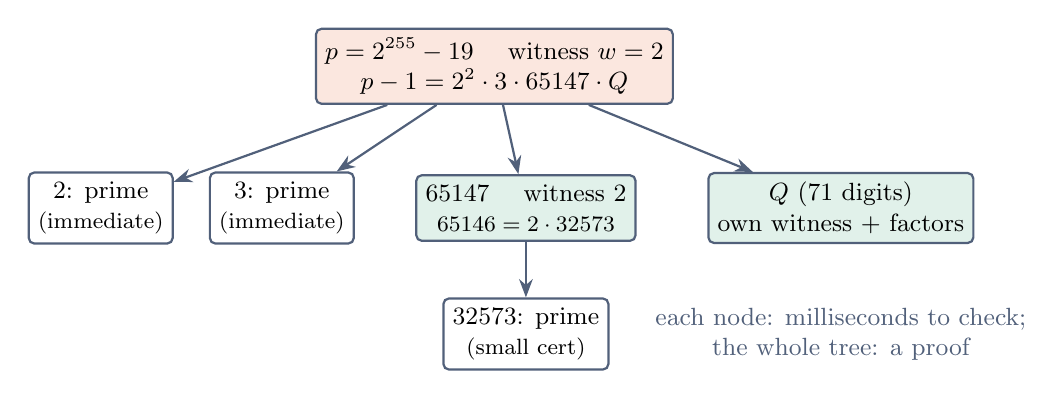
\begin{tikzpicture}[
  lvl/.style={draw=ink2,thick,rounded corners=2pt,fill=white,align=center,font=\small},
  edge/.style={-{Stealth},ink2,thick}
]
  \node[lvl,fill=accentsoft] (p) at (0,2.7)
    {$p = 2^{255}-19$ \quad witness $w=2$\\ $p-1 = 2^2\cdot 3\cdot 65147\cdot Q$};
  \node[lvl] (two)   at (-5.0,0.9) {$2$: prime\\ \footnotesize (immediate)};
  \node[lvl] (three) at (-2.7,0.9) {$3$: prime\\ \footnotesize (immediate)};
  \node[lvl,fill=provensoft] (m) at (0.4,0.9)
    {$65147$ \quad witness $2$\\ \footnotesize $65146 = 2 \cdot 32573$};
  \node[lvl,fill=provensoft] (q) at (4.4,0.9)
    {$Q$ (71 digits)\\ own witness + factors};
  \node[lvl] (sub) at (0.4,-0.7) {$32573$: prime\\ \footnotesize (small cert)};
  \draw[edge] (p) -- (two); \draw[edge] (p) -- (three);
  \draw[edge] (p) -- (m);   \draw[edge] (p) -- (q);
  \draw[edge] (m) -- (sub);
  \node[font=\small\color{ink2},align=center] at (4.4,-0.7)
    {each node: milliseconds to check;\\ the whole tree: a proof};
\end{tikzpicture}
\end{center}

(Check one leaf of this tree yourself right now, no computer:
$4 \cdot 3 \cdot 65147 = 781764$, and $781764 \cdot Q$ must reproduce the
77-digit $p-1$ --- the \emph{product identity} is the easiest condition of
a certificate to audit, and auditing one leaf by hand is a good habit
before trusting a tree. The witness conditions for $w = 2$ at the top node
were re-verified computationally while writing this chapter; the
kernel-checked version of this construction, for the Pallas modulus, lives
in \code{pasta-pallas-verified}.)

\begin{worked}{checking a Pratt certificate by hand --- all of it}
Nothing builds trust in a certificate like verifying one completely, so
here is the full check for $n = 97$, witness $w = 5$ --- every modular
multiplication on this page, using the same square-and-multiply ladder
the real code uses (and which you will implement in the exercises).
First the data: $n - 1 = 96 = 2^5 \cdot 3$, so there are three
conditions: $5^{96} \equiv 1$, $5^{96/2} = 5^{48} \not\equiv 1$, and
$5^{96/3} = 5^{32} \not\equiv 1 \pmod{97}$.

Build the powers of $5$ by repeated squaring mod $97$, reducing as you go
--- each line is one two-digit multiplication and one division with
remainder, nothing more:
\[
\begin{array}{lclcl}
5^{2} &=& 25 \\
5^{4} &=& 25^2 = 625 &=& 6\cdot 97 + 43 \;\to\; 43\\
5^{8} &=& 43^2 = 1849 &=& 19\cdot 97 + 6 \;\to\; 6\\
5^{16} &=& 6^2 &=& 36\\
5^{32} &=& 36^2 = 1296 &=& 13\cdot 97 + 35 \;\to\; 35\\
\end{array}
\]
Now assemble the three exponents from these squares:
\[
5^{48} = 5^{32} \cdot 5^{16} = 35 \cdot 36 = 1260 = 12 \cdot 97 + 96
\;\to\; 96 \equiv -1 ,
\]
\[
5^{96} = (5^{48})^2 \equiv (-1)^2 = 1 . \qquad ✓
\]
Check the conditions: $5^{96} \equiv 1$ ✓; $5^{48} \equiv 96 \neq 1$ ✓;
$5^{32} \equiv 35 \neq 1$ ✓. All three hold --- and by Pratt's theorem
(whose reason the exercises make you articulate), $97$ is prime, with the
whole verification costing \emph{seven} small multiplications. Trial
division would have cost eight test divisions here --- no savings at two
digits. But the ladder's cost grows with the \emph{number of bits} (one
squaring per bit), while trial division grows with the \emph{square root
of the value} (one division per candidate) --- linear versus exponential
in the bit-length. At 77 digits that gap is the whole story, as the next
box counts.
\end{worked}

\begin{worked}{costing the real certificate for $p = 2^{255}-19$}
How much work is the full certificate check for the real prime, versus
trial division? Count it, honestly, using the tree above.

\emph{Certificate side.} One modular exponentiation with a 255-bit
exponent costs at most $254$ squarings plus at most $254$ multiplies ---
call it $\le 508$ modular multiplications, and abbreviate ``modmul.''
The top node needs: $2^{p-1}$ (one exponentiation), and one
$2^{(p-1)/q}$ for each of the four prime factors $q \in \{2, 3, 65147,
Q\}$ --- five exponentiations, $\le 2540$ modmuls. The recursion adds:
$Q$'s own node ($Q-1$ has its own small factor list; generously, another
five exponentiations at 71 digits, $\le 2350$ modmuls), the $65147$ node
(16-bit numbers --- three exponentiations of $\le 32$ modmuls, noise),
and $32573$'s (noise). Round the entire tree up to
\[
\text{certificate check} \;\lesssim\; 5{,}000 \text{ modmuls.}
\]
\emph{Trial division side.} $\sqrt{p} \approx 2^{127.5}$, and candidate
divisors (odd numbers, say) number about $2^{126.5} \approx 10^{38}$.
\emph{Ratio}:
\[
\frac{10^{38} \text{ divisions}}{5 \times 10^{3} \text{ modmuls}}
\;\approx\; 10^{34}.
\]
Thirty-four orders of magnitude --- not an optimization, a different
universe. And one more accounting worth doing: the certificate
\emph{data} is four factor entries and a handful of witnesses --- a few
hundred bytes. Someone (a computer algebra system, years of CPU time,
once, offline) paid dearly to \emph{find} the factorization of $p-1$;
every checker since pays five thousand multiplications. That asymmetry
--- expensive find, cheap check, tiny certificate --- is the shape of
every proof object the Lean kernel will ever hand you.
\end{worked}

\begin{aha}
This find/check asymmetry is one of the great ideas of computer science ---
it is the P versus NP distinction wearing work clothes, and it is the engine
of zero-knowledge proof systems (the very technology the Pasta curves serve).
Proof assistants run on it too: Lean's whole architecture --- clever tactics
\emph{finding}, dumb kernel \emph{checking} --- is the same asymmetry. A
proof \emph{is} a certificate.
\end{aha}

\section{The tempting shortcut, and why the house declines it}

Lean offers a faster \lean{decide}: the variant \lean{native_decide}
compiles the decision procedure to native machine code, runs it at full
speed, and asserts the result. With a good primality test behind it, it can
dispatch \lean{Nat.Prime p} in seconds. Case closed?

Look at what you would be trusting. Ordinary \lean{decide} produces a
computation the \emph{kernel} replays --- the ~few-thousand-line paranoid
core remains the only thing you trust. \lean{native_decide} instead makes
the theorem's truth depend on the Lean \emph{compiler}, the C toolchain
behind it, and the runtime --- hundreds of thousands of lines promoted into
your trusted base, in exchange for convenience on one theorem. Every proof
downstream of the field --- group law, scalars, signatures --- would inherit
that enlarged trust, visible forever in its axiom report
(Chapter~\ref{ch:honesty} shows you how to read those).

\begin{pitfall}
\lean{native_decide} is not ``cheating,'' and for exploratory work it is a
fine tool. The trap is \emph{silent trust inflation}: its use is invisible at
the theorem statement --- the cost appears only when someone audits the
axioms, which is exactly what most readers never do. House rule, adopted from
the projects this book accompanies: exploratory scaffolding may use it;
\textbf{no shipped certificate depends on it}. The final Pallas-modulus
primality proof in \code{pasta-pallas-verified} is a kernel-checked
Lucas/Pratt certificate for precisely this reason.
\end{pitfall}

\section{Certificates in practice: Mathlib's toolbox}

You will not hand-roll witness trees. Mathlib provides the machinery
(\lean{Nat.Prime} decision lemmas, \lean{lucas_lehmer}-style infrastructure,
and the \lean{norm_num} extension \lean{Nat.Prime} plugin) that constructs
and checks Pratt-style certificates behind a single tactic call --- while
keeping every step kernel-checked. The shape in real code:

\begin{lstlisting}[language=Lean]
theorem p_prime : Nat.Prime (2^255 - 19) := by
  norm_num  -- certificate-backed primality, kernel-checked, ~seconds
\end{lstlisting}

When the built-in route struggles (very large or awkward moduli), the
fallback is explicit: state the witness data as definitions, prove the two
Pratt conditions with \lean{norm_num}-driven modular exponentiation, and
assemble. That is exactly the structure of the Pallas certificate in the
companion repository --- worth reading now with fresh eyes:
\code{pasta-pallas-verified/verification/Proofs/Primality.lean}.

\begin{tryit}
Open \code{exercises/Ch07.lean}. Ladder: certify $97$, then $65537$ (a
Fermat prime beloved of RSA), then the ten-digit Mersenne prime $2^{31}-1$,
watching what each tool costs as the numbers grow. (Amusingly, the
find/check asymmetry bites the \emph{tactic} too: \lean{norm_num} must
\emph{find} the witness tree before the kernel checks it, and at $2^{61}-1$
the finding already takes minutes.) Finale: implement square-and-multiply
modular exponentiation yourself and check the top witness condition for
$p = 2^{255}-19$ with \lean{\#eval} --- your own hands on the certificate,
at 77 digits, in milliseconds.
\end{tryit}

\section*{Exercises}

\exercise{Verify by hand that $w = 2$ is a Pratt witness for $p = 13$:
compute $2^{12} \bmod 13$ and $2^{12/q} \bmod 13$ for each prime $q \mid 12$.
Write the full certificate tree for $13$, recursing into the factors of
$12$.}

\exercise{Why does the witness condition force primality? Sketch the
argument: if $w$ has order exactly $p-1$ in $\Zmod{p}$, then the
multiplicative structure has $p-1$ elements, which fails if $p = ab$ with
$1 < a,b < p$. (Full rigor optional; the shape is the point.)}

\exercise{(Paper) Certify $65147$ by hand-checkable data: given
$65146 = 2 \cdot 32573$ and witness $w = 2$, list the exact conditions a
checker must verify, then carry out the \emph{cheapest} one:
$2^{65146/32573} = 2^2 = 4 \not\equiv 1 \pmod{65147}$. For the remaining
two conditions, count precisely how many squarings and multiplications the
ladder needs (do not perform them). How many two-to-five-digit
multiplications, total, stand between a skeptic and certainty about
$65147$?}

\exercise{(Discussion) Bitcoin miners \emph{find} block hashes; nodes
\emph{check} them. GPS receivers \emph{check} satellite signals they could
never \emph{find}. Name two more systems built on the find/check asymmetry,
and one system that would collapse without it.}

\section*{Solutions and pathways}
\solutionsintro

\solhead{7.1}
\pathway The data first: $12 = 2^2 \cdot 3$, so two conditions beyond
$w^{12} \equiv 1$: exponents $12/2 = 6$ and $12/3 = 4$. Then power up $2$
mod $13$ by successive squaring, as the worked example did for $97$ ---
at this size you can even go linearly.
\answer Powers of $2$ mod $13$: $2^2 = 4$, $2^4 = 16 \equiv 3$,
$2^6 = 2^4 \cdot 2^2 = 3 \cdot 4 = 12 \equiv -1$, and
$2^{12} = (2^6)^2 \equiv (-1)^2 = 1$. Conditions: $2^{12} \equiv 1$ ✓;
$2^{6} \equiv 12 \neq 1$ ✓; $2^{4} \equiv 3 \neq 1$ ✓. Witness confirmed.
The full tree: node $13$ (witness $2$, $12 = 2^2 \cdot 3$) with children
$2$ (immediate) and $3$ (witness $2$: $2^2 = 4 \equiv 1 \pmod 3$, and
$2^{2/2} = 2 \not\equiv 1$ --- a two-line sub-certificate). Every claim in
the tree is now something you have personally multiplied.

\solhead{7.2}
\pathway The key concept is the \emph{order} of $w$: the least $e > 0$
with $w^e \equiv 1$. The two witness conditions pin the order exactly;
then count invertible elements two ways.
\answer The condition $w^{p-1} \equiv 1$ says the order of $w$ divides
$p-1$; the conditions $w^{(p-1)/q} \not\equiv 1$ for every prime
$q \mid p-1$ rule out every \emph{proper} divisor of $p-1$ (any proper
divisor of $p-1$ divides some $(p-1)/q$). So the order is exactly $p-1$:
the powers $w^1, w^2, \dots, w^{p-1}$ are $p-1$ \emph{distinct} elements,
all invertible mod $p$ (each has $w^{\text{something}}$ as inverse). But
if $p = ab$ with $1 < a, b < p$, the element $a$ is a zero divisor ---
$a \cdot b \equiv 0$ --- so $a$ is not invertible, and neither are its
multiples: strictly fewer than $p-1$ residues can be invertible.
Contradiction; $p$ has no such factorization. (Full rigor pins down
``distinct'' and the divisor-covering claim --- both one-liners with the
order concept in hand. The shape is: \emph{one loud element forces the
whole multiplicative structure to be as big as only a prime allows.})

\solhead{7.3}
\pathway List conditions mechanically from the definition, then count
ladder steps: an exponent of $b$ bits costs $\le b-1$ squarings plus (at
worst) $b-1$ multiplies; $65146 < 2^{16}$ and $32573 < 2^{15}$.
\answer Conditions: (i) $2^{65146} \equiv 1 \pmod{65147}$;
(ii) $2^{65146/2} = 2^{32573} \not\equiv 1$;
(iii) $2^{65146/32573} = 2^{2} = 4 \not\equiv 1$ ✓ (done --- four is
visibly not one); plus the recursive certificate for $32573$. Counting:
$65146$ has $16$ bits ($2^{16} = 65536$), so condition (i) costs $\le 15$
squarings $+ \le 15$ multiplies $= 30$; condition (ii), $15$ bits,
$\le 28$; condition (iii) was free. Sub-certificate for $32573$
($32572 = 2^2 \cdot 17 \cdot 479$): four conditions on $\le 15$-bit
exponents, $\le 4 \cdot 28 = 112$, plus leaves ($17$, $479$ ---
another $\sim 60$ generously). Total: \emph{under $250$ small
multiplications} --- an afternoon with paper, an eyeblink for a kernel,
and at the end $65147$ is not ``probably prime'' but \emph{prime}. (For
the audit-minded: you were given $32572$'s factorization here the same
way the checker is --- as certificate data. Verifying
$4 \cdot 17 \cdot 479 = 32572$ is one more hand multiplication:
$68 \cdot 479 = 32572$ ✓.)

\solhead{7.4}
\pathway Look for systems where producing an artifact is costly but a
short receipt convinces everyone --- then for the collapse case, imagine
checking costing as much as finding.
\answer (Model answers.) Two more: \emph{academic peer review of
computer-assisted proofs} --- the four-color theorem's checkers verify in
hours what took years to construct; and \emph{password hashing} ---
deriving a hash from a password is instant to check against, infeasible
to invert. Others students propose: sudoku (solve vs.\ check), lottery
tickets (draw vs.\ verify), digital signatures themselves (sign with
secret effort-equivalent, verify publicly). A system that would collapse
without the asymmetry: \emph{blockchain consensus} --- if verifying a
block cost as much as mining it, every node would need a mine's
electricity bill and the network could not exist. (So would mathematics
as a social enterprise: if checking a proof cost as much as finding it,
referees would be as rare as authors. In a sense, Lean is what happens
when you drive the check cost toward zero and let anyone be a referee.)

\begin{checkpoint}
You should now be able to: explain why \lean{decide} cannot prove
$2^{255}-19$ prime while a certificate can; reproduce the two Pratt witness
conditions and check them on a small prime; articulate exactly what
additional trust \lean{native_decide} would introduce and why shipped
certificates decline it; and recognize the find/check asymmetry as the
common engine of certificates, proof assistants, and the P-vs-NP question.
\end{checkpoint}

\chapter{From Rust to Lean: Verifying the Code That Actually Ships}
\label{ch:rust}

\section{The transcription problem}

Everything so far proved facts about \emph{Lean} programs. But the Ed25519
that guards your SSH connection is written in \emph{Rust} (in our case,
\code{curve25519-dalek} and its forks). An obvious plan: read the Rust,
rewrite it in Lean by hand, verify the rewrite. The plan has a hole you could
drive a key-recovery attack through: \textbf{what if you transcribe it
wrong?} A hand-copy that silently fixes a bug --- or introduces one --- makes
the proof a beautiful statement about code nobody runs.

The projects behind this book close the hole with a mechanical translation
pipeline:

\begin{center}
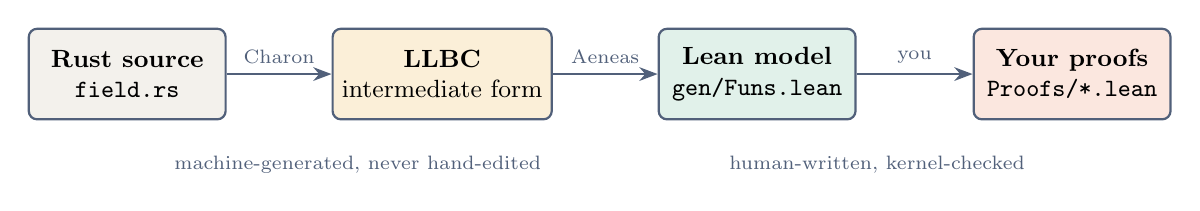
\begin{tikzpicture}[
  stage/.style={draw=ink2,thick,rounded corners=3pt,align=center,
                minimum height=1.15cm,minimum width=2.5cm,font=\small},
  arr/.style={-{Stealth},thick,ink2},
  lbl/.style={font=\scriptsize\color{ink2},midway,above}
]
  \node[stage,fill=codebg]     (rust)  at (0,0)    {\textbf{Rust source}\\ \code{field.rs}};
  \node[stage,fill=warnsoft]   (llbc)  at (4.0,0)  {\textbf{LLBC}\\ intermediate form};
  \node[stage,fill=provensoft] (model) at (8.0,0)  {\textbf{Lean model}\\ \code{gen/Funs.lean}};
  \node[stage,fill=accentsoft] (proof) at (12.0,0) {\textbf{Your proofs}\\ \code{Proofs/*.lean}};
  \draw[arr] (rust)  -- node[lbl]{Charon}  (llbc);
  \draw[arr] (llbc)  -- node[lbl]{Aeneas}  (model);
  \draw[arr] (model) -- node[lbl]{you}     (proof);
  \node[font=\scriptsize\color{ink2},align=center] at (6.0,-1.15)
    {machine-generated, never hand-edited \hspace{2.2cm} human-written, kernel-checked};
\end{tikzpicture}
\end{center}

\textbf{Charon} compiles the Rust crate into LLBC (``low-level borrow
calculus''), a simplified intermediate representation. \textbf{Aeneas}
translates LLBC into pure Lean functions. The generated Lean --- the
\emph{model} --- lands in a \code{gen/} directory with a strict house rule:
\emph{never edit it}. Regenerate it from source, or don't touch it. Your
proofs import the model and state theorems about it.

\begin{bigidea}
The object of verification is the \textbf{extracted model}, produced from
the shipping source by a deterministic tool --- not a human transcription.
The trust question shifts from ``did we copy the code right?'' (unauditable
squinting) to ``does the translator preserve meaning?'' (one tool, studied
once, shared by every project that uses it). You will hear this called
\emph{shrinking the trusted base}: swap many ad-hoc trusts for one
well-examined trust.
\end{bigidea}

\section{What extracted code looks like}

Here is real input and real output, lightly abridged. The Rust (from
\code{curve25519-dalek}, radix-51 field addition):

\begin{lstlisting}[language=RustL]
impl Add for FieldElement51 {
    fn add(self, rhs: &FieldElement51) -> FieldElement51 {
        let mut output = *self;
        for i in 0..5 {
            output.0[i] += rhs.0[i];
        }
        output
    }
}
\end{lstlisting}

And the Lean model Aeneas produces for it (shape, not verbatim):

\begin{lstlisting}[language=Lean]
def fieldElement51_add (self rhs : Array U64 5) :
    Result (Array U64 5) := do
  let a0 <- Array.index_usize self 0
  let b0 <- Array.index_usize rhs 0
  let s0 <- a0 + b0            -- U64 addition: can FAIL on overflow
  let out <- Array.update self 0 s0
  ...                          -- and so on for limbs 1..4
\end{lstlisting}

Three features deserve your full attention, because every proof in the next
two chapters engages them:

\begin{itemize}[leftmargin=1.4em]
\item \textbf{Machine integers are honest.} \lean{U64} is not $\N$; it is
  64-bit words. Aeneas models arithmetic on them precisely, overflow
  included.
\item \textbf{Everything returns \lean{Result}.} The \lean{do}/\lean{<-}
  notation threads a computation that can \emph{fail} --- returning an error
  value instead of a result --- exactly where the Rust could panic or
  overflow. There is no pretending partial functions are total.
\item \textbf{It is ugly.} Five limbs times load-add-store, all sequenced.
  Machine-generated code has no taste. The \emph{proofs} restore the
  elegance; the model's job is fidelity.
\end{itemize}

\section{Overflow is a proof obligation, not a footnote}

In Rust, \rust{a + b} on \rust{u64} panics in debug mode and wraps in
release mode when it overflows. In the extracted model, \lean{a + b}
returns a \lean{Result} that is an error unless the mathematical sum fits.
So the innocent theorem ``add returns the right field element'' \emph{cannot
even be stated} without first proving \emph{add returns at all}:

\begin{lstlisting}[language=Lean]
theorem add_spec (a b : Array U64 5)
    (ha : LimbsBounded a) (hb : LimbsBounded b) :
    ∃ c, fieldElement51_add a b = .ok c ∧ LimbsBounded c ∧ ...
\end{lstlisting}

That hypothesis \lean{LimbsBounded} --- each limb below $2^{54}$, say --- is
the bounds invariant promised in Chapters~\ref{ch:pat}
and~\ref{ch:modular}: 51-bit payload plus headroom, so limb additions cannot
reach $2^{64}$. The specification exposes what the Rust comments only
whisper: this code is correct \emph{under a discipline of bounded inputs},
the discipline must be maintained by every caller, and now there is a
machine checking that it is.

\begin{aha}
Notice what just happened to ``ugly generated code with Results
everywhere'': it forced us to discover, state, and prove the \emph{implicit
operating envelope} of the optimized implementation. The dalek authors knew
this envelope; it lived in comments and code-review lore. Now it is a
theorem. Extraction does not merely enable verification --- it
\emph{interrogates} the code.
\end{aha}

\section{Practicalities: extraction as surgery}

Running Charon on a whole real-world crate drags in everything the crate
touches --- iterators, byte serialization, trait machinery, SIMD backends
--- much of it irrelevant to the arithmetic core and some of it beyond what
the translator supports. The working method, learned the honest way in the
companion projects:

\begin{itemize}[leftmargin=1.4em]
\item \textbf{Extract functions, not crates.} Charon accepts specific roots
  (individual functions and impls); the extraction scripts in each companion
  repo (\code{extract.sh}, \code{extract-scalar.sh}) name exactly the
  arithmetic functions and get a small, clean model --- 28 definitions
  instead of a thousand.
\item \textbf{Some code will not translate.} The dalek scalar-multiplication
  backends use CPU-specific SIMD intrinsics no translator models. The
  boundary is then \emph{documented}: those functions enter the trusted base,
  stated as assumptions, visible in every audit. Honest boundaries beat
  heroic fictions (Chapter~\ref{ch:honesty} dwells on this).
\item \textbf{Pin your tools.} The pipeline records exact versions of
  Charon, Aeneas, and Lean. A model regenerated with a different translator
  version is a \emph{different model}; reproducibility of the proofs starts
  with reproducibility of the artifact under proof.
\end{itemize}

\begin{pitfall}
When an extraction fails or a model looks bizarre, the temptation is to
``fix'' the generated Lean by hand. Resist absolutely. A hand-edited model
is a hand-transcription with extra steps --- the exact hole this pipeline
exists to close. The fixes live in extraction scope (choose different
roots), in the source (rarely), or in documented assumptions (openly).
\end{pitfall}

\begin{tryit}
Open the companion repo \code{dalek-ed25519-verified}: read
\code{extract.sh} (the roots), skim \code{verification/gen/Funs.lean} for
\code{add}/\code{sub} (recognize the load-add-store pattern above), then
read the first twenty lines of \code{verification/Proofs/FieldSpec.lean}
and identify: the bounds invariant, the \lean{Result} handling, and the
statement of the theorem. You now recognize every structural element. The
mathematics inside is Chapters~\ref{ch:denotation} and~\ref{ch:field}.
\end{tryit}

\section*{Exercises}

\exercise{The Rust expression \rust{output.0[i] += rhs.0[i]} hides four
distinct failure/effect points that the Lean model makes explicit. Name
them. (Hint: two indexings, one arithmetic operation, one write.)}

\exercise{Suppose limbs are bounded by $2^{54}$. What is the largest value
\lean{a0 + b0} can take, and how many such additions can chain before a
\lean{U64} overflow becomes possible? Show the margin calculation --- this
is precisely why the invariant is $2^{54}$ and not $2^{63}$.}

\exercise{(Design) Your colleague proposes verifying a hand-written Lean
``reference implementation'' instead of the extracted model, because it is
prettier. List two failure modes this reintroduces, and one legitimate use a
reference implementation still has (hint: Chapter~\ref{ch:denotation} uses
one as the \emph{specification} side).}

\begin{checkpoint}
You should now be able to: draw the Rust $\to$ LLBC $\to$ Lean pipeline and
say what each stage preserves; explain why generated models are never
hand-edited; read a \lean{Result}-typed extracted function and point to
where overflow lives; and state why ``the proof needs a bounds hypothesis''
is a discovery about the \emph{code}, not a weakness of the method.
\end{checkpoint}

\chapter{The Denotation Bridge: What Do Five Numbers \emph{Mean}?}
\label{ch:denotation}

\section{Two worlds, one bridge}

We now hold two very different objects. On one side, mathematics:
the field $\Fp$, where elements are abstract clock positions and $+$ means
ideal modular addition. On the other side, the extracted model: arrays of
five \lean{U64} words, shuffled by loads, adds, and stores. The entire
question of verified cryptography is how to say --- precisely --- that the
second \emph{implements} the first.

The answer is a single function, small enough to write on one line and
important enough to carry this whole book. Given limbs
$a = (a_0, a_1, a_2, a_3, a_4)$, define the \textbf{denotation}:
\[
\denote{a} \;=\; a_0 + 2^{51} a_1 + 2^{102} a_2 + 2^{153} a_3 + 2^{204} a_4
\;\in\; \Fp .
\]
Read $\denote{a}$ as ``the field element these limbs \emph{mean}.'' It is
positional notation, nothing more --- base $2^{51}$ instead of base 10, with
the result interpreted on the clock face of $\Fp$. In Lean:

\begin{lstlisting}[language=Lean]
def denote (a : Array U64 5) : ZMod p :=
  a[0].val + 2^51 * a[1].val + 2^102 * a[2].val
           + 2^153 * a[3].val + 2^204 * a[4].val
\end{lstlisting}

With the bridge in hand, correctness of an operation becomes a
\emph{commuting square} --- one picture you should internalize until you see
it in your sleep:

\begin{center}
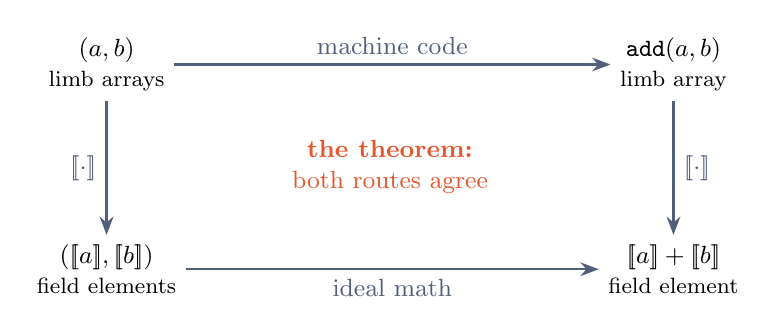
\begin{tikzpicture}[
  world/.style={font=\small,align=center},
  arr/.style={-{Stealth},thick,ink2},
  lbl/.style={font=\small\color{ink2}}
]
  \node[world] (tl) at (0,2.6)   {$(a, b)$\\ \footnotesize limb arrays};
  \node[world] (tr) at (7.2,2.6) {$\mathtt{add}(a,b)$\\ \footnotesize limb array};
  \node[world] (bl) at (0,0)     {$(\denote{a}, \denote{b})$\\ \footnotesize field elements};
  \node[world] (br) at (7.2,0)   {$\denote{a} + \denote{b}$\\ \footnotesize field element};
  \draw[arr] (tl) -- node[lbl,above] {machine code} (tr);
  \draw[arr] (bl) -- node[lbl,below] {ideal math} (br);
  \draw[arr] (tl) -- node[lbl,left]  {$\denote{\cdot}$} (bl);
  \draw[arr] (tr) -- node[lbl,right] {$\denote{\cdot}$} (br);
  \node[font=\small\color{accent},align=center] at (3.6,1.3)
    {\textbf{the theorem:}\\ both routes agree};
\end{tikzpicture}
\end{center}

\begin{bigidea}
\textbf{The correctness of an implementation is the statement that
denotation commutes with every operation:}
\[
\denote{\mathtt{add}(a,b)} = \denote{a} + \denote{b},
\qquad
\denote{\mathtt{mul}(a,b)} = \denote{a} \cdot \denote{b},
\qquad\dots
\]
The left-hand side lives in the machine world (with its bounds hypotheses
and \lean{Result}s); the right-hand side is pure mathematics. One equation
per operation, and the ugly optimized code is pinned, forever, to the
textbook meaning. Every verified-crypto project you will ever read is this
diagram, instantiated.
\end{bigidea}

\section{Why redundancy is freedom (and where bugs hide)}

A subtlety with consequences: denotation is \textbf{many-to-one}. The limb
arrays $(19, 0, 0, 0, 0)$ and $(p + 19 \bmod 2^{\cdots}, \dots)$ --- or more
mundanely, unreduced sums whose limbs exceed $2^{51}$ --- can denote the
\emph{same} field element. The representation has slack, and the
implementation \emph{exploits} it: the fast \code{add} from
Chapter~\ref{ch:rust} just adds limbs pairwise, letting values drift above
$2^{51}$, and nobody reduces until a cheaper moment. The commuting square
still closes because $\denote{\cdot}$ doesn't care how bloated the limbs are
--- positional value is positional value.

This is also exactly where the carry bugs of Chapter~\ref{ch:why} live: code
that is correct only while the drift stays within headroom, and wrong on the
rare inputs where it spills. In the verified development that danger becomes
a visible, machine-checked pair of clauses attached to every operation:

\begin{lstlisting}[language=Lean]
theorem add_spec (ha : Bnd54 a) (hb : Bnd54 b) :
    ∃ c, add a b = .ok c
       ∧ Bnd55 c                        -- (1) bounds: the envelope holds
       ∧ denote c = denote a + denote b -- (2) value: the meaning is right
\end{lstlisting}

Clause (2) is the commuting square. Clause (1) feeds the \emph{next}
operation's hypothesis --- correctness composes only because every theorem
hands the following one the envelope it requires. A chain of such specs is
the formal skeleton of ``this sequence of optimized operations computes the
formula we claim.''

\begin{aha}
The denotation idea is vastly older and bigger than cryptography. Compilers
prove ``optimized code means the same as naive code''; databases prove
``this query plan means the same query''; hardware verifies ``this pipelined
circuit means this instruction set.'' The pattern --- map both sides into a
mathematical meaning-space and prove the square commutes --- is called
\emph{denotational semantics}, and you have now used it for real. It is the
single most transferable idea in this book.
\end{aha}

\section{Multiplication: where the bridge earns its keep}

Addition's square closes in an afternoon. Multiplication is the boss fight,
and seeing \emph{why} teaches you what verified arithmetic is really like.
Schoolbook multiplication of two 5-limb numbers produces nine columns of
partial products $\sum_{i+j=k} a_i b_j$; each column then owes a
\emph{carry} to the next; and columns $k \ge 5$ --- weights $2^{255}$ and up
--- must be folded back using the Chapter~\ref{ch:modular} identity
$2^{255} \equiv 19$. The implementation interleaves all three concerns for
speed. The proof must un-interleave them:

\[
\denote{\mathtt{mul}(a,b)}
\;\overset{?}{=}\;
\Big(\textstyle\sum_{k=0}^{8} 2^{51k} \sum_{i+j=k} a_i b_j \Big) \bmod p
\;\overset{?}{=}\; \denote{a} \cdot \denote{b} .
\]

The right equality is algebra --- \lean{ring} territory. The left is a walk
through the extracted code: every intermediate \lean{U128} product bounded
(no overflow --- the $2^{54}$ headroom at work), every carry accounted,
every $\times 19$ fold placed. In the companion projects this is a long
\lean{calc}-and-\lean{have} museum: dozens of small steps, each dispatched
by \lean{omega} or a bound lemma, composed into one commuting square.

One more representational dialect, because you will meet it in the Pasta
repos: \textbf{Montgomery form} stores $x$ as $x \cdot R \bmod p$ (with
$R = 2^{256}$) because it makes reduction after multiplication cheap. The
bridge absorbs the twist without complaint --- define
$\denote{a}_{\mathrm{M}} = (\text{positional value of } a) \cdot R^{-1}$
and the same commuting squares govern everything. Denotation is a
\emph{policy about meaning}, and it bends to fit the representation, not
the other way around.

\begin{pitfall}
When a denotation proof refuses to close, the failure is information ---
read it like a detective, in order: (1) Is the \emph{bound} hypothesis
strong enough for the intermediate products? (Count bits, on paper.)
(2) Is the \emph{denotation} right for this representation --- radix, limb
count, Montgomery factor? (3) Only then suspect the code. In the companion
projects this checklist ran hundreds of times; its order reflects the actual
base rates of what was wrong.
\end{pitfall}

\begin{tryit}
Open \code{exercises/Ch09.lean}. It builds a miniature of the whole story
you can hold in your head: a \emph{2-limb, radix-4} representation of
$\Zmod{15}$ (limbs are values $0$--$3$, denotation $a_0 + 4a_1$, and
$16 \equiv 1$ makes the fold trivial). You will write \lean{denote}, prove
the commuting square for the provided \lean{add} with carry, then for
\lean{mul} with its fold --- every conceptual ingredient of the dalek proof,
at a scale where \lean{decide} can double-check your work.
\end{tryit}

\section*{Exercises}

\exercise{Compute by hand the denotation of the limb arrays $(19,0,0,0,0)$
and $(0,0,0,0,2^{51})$ in the radix-51 system, reducing mod $p = 2^{255}-19$.
Conclude that $\denote{\cdot}$ is not injective by exhibiting the collision.}

\exercise{In the mini-system of the Try It box, find two distinct limb pairs
denoting the same element of $\Zmod{15}$, and check that the provided
\lean{add} treats them interchangeably \emph{as far as denotation goes} ---
compute both sides.}

\exercise{Sketch the multiplication column sums $\sum_{i+j=k} a_i b_j$ for
the 2-limb system and carry out the fold $16 \equiv 1$ by hand for
$a = (3,2)$, $b = (1,3)$. Check against direct computation in $\Zmod{15}$.}

\exercise{(Paper, challenge) For the radix-51 system with limbs bounded by
$2^{54}$: bound one column $\sum_{i+j=4} a_i b_j$ of partial products and
confirm it fits a \lean{U128}. How much headroom remains? This number ---
not elegance --- is why the invariant chose $2^{54}$.}

\begin{checkpoint}
You should now be able to: write the radix-51 denotation from memory; draw
the commuting square and label which side owns bounds and \lean{Result}s;
explain why many-to-one representation is both the performance trick and
the bug habitat; and recognize the two-clause shape (bounds propagation +
value equation) as the universal skeleton of implementation-correctness
theorems.
\end{checkpoint}

\chapter{Verifying a Field: The Full Campaign}
\label{ch:field}

\section{The summit statement}

Every thread so far --- specs as types, tactics, automation, $\Fp$,
primality, extraction, denotation --- was preparation for one theorem. In
the companion repositories it is called the \emph{field implementation
certificate}, and (lightly paraphrased) it says:

\begin{lstlisting}[language=Lean]
theorem fieldImplementation :
    -- p is prime, so ZMod p is genuinely a field
    Nat.Prime p
    -- and for all bounded limb arrays, every operation's
    -- commuting square closes:
  ∧ (∀ a b, Bnd a → Bnd b → AddSquare a b)
  ∧ (∀ a b, Bnd a → Bnd b → SubSquare a b)
  ∧ (∀ a b, Bnd a → Bnd b → MulSquare a b)
  ∧ (∀ a,   Bnd a →         SquareSquare a)
  ∧ (∀ a,   Bnd a →         InvertSquare a)   -- Fermat chain: a^(p-2)
  ∧ ...                                       -- reduce, negate, encode
\end{lstlisting}

One theorem, kernel-checked, quantified over \emph{every} input the
representation admits: the extracted dalek field arithmetic implements
$\Fp$. This chapter is the story of the campaign that proves it --- told
honestly, including the two places where the terrain fought back, because
the failures teach more than the victories.

\section{Order of battle}

You do not prove such a conjunction by heroism; you prove it by sequencing.
The campaign order in the real projects, and the reason for each position:

\begin{enumerate}[leftmargin=1.6em]
\item \textbf{Bounds lemmas first} --- pure \lean{omega} facts about limb
  sizes, no denotation at all. Cheap, and everything depends on them.
\item \textbf{Primality} (Chapter~\ref{ch:prime}) --- independent of the
  code entirely; it dignifies \lean{ZMod p} into a field.
\item \textbf{add, sub, negate} --- linear operations; the commuting squares
  close with \lean{omega} plus the denotation unfolds. Confidence builders.
\item \textbf{reduce} --- the $\times 19$ fold in isolation. Proving it
  alone, before mul uses it, halves the hardest proof's size.
\item \textbf{mul, square} --- the boss fight of Chapter~\ref{ch:denotation}:
  column sums, carries, folds. Squaring is mul with algebraic shortcuts ---
  a separate code path in dalek, hence a separate theorem. No shortcuts
  in the proof: the \emph{code's} shortcut is precisely what needs checking.
\item \textbf{invert} --- the 254-squaring Fermat chain, verified as a
  \lean{calc} of exponent bookkeeping on top of \code{mul}/\code{square}
  specs, ending at $a^{p-2}$; Fermat's little theorem (Mathlib's) closes
  the square.
\end{enumerate}

Notice the shape: \emph{each layer consumes only the specs of the layer
below}, never reaching into implementations. By step 6 you are doing exponent
arithmetic, blissfully ignorant of carries. That is the compositionality that
Chapter~\ref{ch:denotation}'s two-clause specs (bounds + value) were designed
to buy.

\begin{worked}{why $16p$ --- auditing a design constant to the bit}
Step 3's subtraction hides the field layer's most quotable design
decision, and you can audit it completely. The problem: compute $a - b$
limb-wise in unsigned words, where limbs of $b$ may be as large as
$2^{54} - 1$ (the invariant's edge) while limbs of $a$ may be as small as
$0$. Unsigned subtraction would truncate (Chapter~\ref{ch:lean}); the fix
is to compute $a + (kp - b)$ for a suitable multiple $k$ of the prime ---
denotationally free, since $kp \equiv 0$ --- chosen so that every limb of
$kp - b$ stays positive. How large must $k$ be? The limb constants of
$kp$ scale the telescoped representation from Chapter~\ref{ch:denotation}:
\[
kP = \big(k(2^{51}-19),\; k(2^{51}-1),\; k(2^{51}-1),\; k(2^{51}-1),\;
k(2^{51}-1)\big),
\]
whose \emph{smallest} limb is $k(2^{51} - 19)$. Positivity of every limb
of $kp - b$ demands
\[
k\,(2^{51} - 19) \;\ge\; 2^{54} - 1 .
\]
Try the candidates, because powers of two are what the code wants:
\[
k = 8:\quad 8(2^{51}-19) = 2^{54} - 152 \;<\; 2^{54} - 1
\qquad\text{✗ fails, by 151;}
\]
\[
k = 16:\quad 16(2^{51}-19) = 2^{55} - 304 \;\ge\; 2^{54} - 1
\qquad\text{✓ with } 2^{54} - 303 \text{ to spare.}
\]
So $16$ is the \emph{least} power of two that works --- $8$ misses by a
margin of $151$, invisible to any test that doesn't drive a limb of $b$
within $151$ of the very top of its envelope. Two more checks complete
the audit: the result's limbs are bounded by
$2^{54} + 2^{55} < 2^{56} < 2^{64}$ (no overflow on the additive side ✓),
and the denotation shifts by exactly $16p \equiv 0$ ✓. In the shipped
proof this box is one lemma with three \lean{omega} obligations; in the
git history of more than one real crypto library, the analogous constant
is a patched CVE. Now you know how to tell which side of that line a
codebase is on.
\end{worked}

\begin{worked}{verifying the inversion chain's bookkeeping --- all 265 steps}
Step 6 sounds heroic --- verify a hand-crafted chain of $254$ squarings
and $11$ multiplications computes $a^{p-2}$ --- until you see that the
whole verification is \emph{exponent arithmetic}, and the exponents obey
one identity you can check at every scale. The chain builds values
$a^{e}$ for a cascade of exponents $e$; squaring doubles $e$, multiplying
adds them. The dalek chain's opening moves:
\[
\begin{array}{lcl}
z_2 = a^2 & & e = 2\\
z_9 = (z_2)^{2^2} \cdot a & & e = 2\cdot 4 + 1 = 9\\
z_{11} = z_9 \cdot z_2 & & e = 9 + 2 = 11\\
z_{2^5-1} = (z_{11})^{2} \cdot z_9 & & e = 22 + 9 = 31 = 2^5 - 1 .
\end{array}
\]
From $31 = 2^5 - 1$ the chain climbs by a doubling ladder whose single
identity you should verify once symbolically:
\[
(2^k - 1)\cdot 2^k + (2^k - 1) \;=\; 2^{2k} - 1
\qquad\text{(``shift a block of $k$ ones up by $k$ and fill'').}
\]
Check it at $k=5$: $31 \cdot 32 + 31 = 992 + 31 = 1023 = 2^{10}-1$ ✓.
The ladder then assembles mixed blocks the same way:
$2^{10}-1 \to 2^{20}-1 \to 2^{40}-1$, then
$(2^{40}-1)2^{10} + (2^{10}-1) = 2^{50}-1$, then
$2^{100}-1 \to 2^{200}-1$, then
$(2^{200}-1)2^{50} + (2^{50}-1) = 2^{250}-1$. Final move: shift five and
add the stashed $z_{11}$:
\[
(2^{250}-1)\cdot 2^{5} + 11 \;=\; 2^{255} - 32 + 11 \;=\; 2^{255} - 21
\;=\; p - 2 . \qquad ✓
\]
Every line above is hand-checkable, and together they \emph{are} the
correctness of the inversion chain --- modulo only ``squaring squares and
multiplication adds exponents,'' which is the already-proven \code{mul}
and \code{square} specs feeding Fermat (Chapter~\ref{ch:modular}). Count
the cost while you are here. Squarings, stage by stage:
$1$ (to $z_2$) $+\,2$ (to $z_9$) $+\,1$ (to $z_{31}$) $+\,5+10+20$ (to
$2^{10},2^{20},2^{40}$) $+\,10$ (to $2^{50}$) $+\,50+100$ (to
$2^{100},2^{200}$) $+\,50$ (to $2^{250}$) $+\,5$ (final shift)
$= 254$. Multiplications: one per block-join --- count the ``$\cdot$''s
above --- exactly $11$. The advertised $254 + 11$ is not folklore; you
just audited it. That is the point of this box: ``verify 265 field
operations'' collapsed into ten lines of exponent algebra a patient
undergraduate audits over coffee.
\end{worked}

\section{Dispatches from the terrain}

\textbf{The wall that was really there.} Partway up, one proof style hit a
genuine limit of the tool: correctness certificates for \code{mul}-scale
goals, when handed to a general decision procedure in one monolithic call,
generate internal certificates with coefficients on the order of $2^{256}$
--- and checking them can exhaust the proof checker's memory. One such call,
during the development of the Pasta field proofs, consumed twelve gigabytes
and crashed the machine (Chapter~\ref{ch:automation} told you this story
from the tactic side). The cure was never cleverness --- it was
\emph{decomposition}: isolate each carry step as its own small lemma with a
tiny context, prove the value identity with \lean{linear_combination}
(a tactic that checks a \emph{stated} linear certificate rather than
searching for one), and let the big theorem be an assembly of small
checked parts. The same discipline, plus hard memory caps on the checker
process, became house infrastructure.

\begin{worked}{the wall, quantified --- why the monolithic proof dies}
The memory catastrophe is not mystical; you can estimate it on one page,
and the estimate teaches the cure. When a decision procedure like
\lean{omega} proves a linear goal, it does not just say ``true'' --- it
emits a \emph{certificate}: a linear combination of the hypotheses with
explicit integer coefficients that the kernel then re-checks
(Chapter~\ref{ch:prime}'s find/check split, again). Now count what a
\emph{monolithic} field-multiplication goal hands it. The goal relates
quantities at wildly different scales: raw limbs ($\sim 2^{51}$), column
sums ($\sim 2^{111}$), folded values ($\sim 2^{116}$), and the final
positional stack, whose top weight is $2^{204}$ --- so eliminating
variables across the whole system produces certificate coefficients up
to the \emph{products} of these scales: numbers of order $2^{256}$ to
$2^{512}$, i.e.\ integers of $80$--$150$ decimal digits. Per
coefficient that is only tens of bytes --- but the elimination is
quadratic-ish in the hypothesis count: with $\sim 60$ hypotheses (five
limbs each for two inputs, nine columns, nine carries, plus bounds for
everything), the certificate and the kernel's intermediate terms
multiply into \emph{millions} of big-number nodes, each participating
in further products. Twelve gigabytes is not even surprising once you
draw the multiplication table of scales --- and this estimate, run
\emph{before} the tactic, is how the wall gets predicted rather than
hit.

The cure now reads directly off the arithmetic: cut the elimination
range. Prove each carry step as its \emph{own} lemma with only its own
few hypotheses in scope (coefficients stay near the step's own scale);
where a large linear identity is genuinely needed, state it yourself
and let \lean{linear_combination} \emph{check} your stated certificate
instead of searching for one (checking is cheap; finding at scale was
the memory bomb). The companion repos' rule --- no blanket automation
in fat contexts --- is this box, written as policy. And note the shape
of the lesson: it is the \emph{same} headroom discipline as the code's
(bound your intermediates, spend your budget consciously), applied one
level up, to the proof itself.
\end{worked}

\begin{aha}
There is a deep symmetry in that fix worth savoring: the \emph{proof} was
restructured exactly the way the \emph{code} was --- into small steps with
controlled intermediate size. Delayed carries in the implementation; small
lemmas in the verification. Bounded limbs; bounded contexts. Good proofs and
good fast code turn out to obey the same engineering aesthetics. This is not
a coincidence; both are fighting combinatorial growth with structure.
\end{aha}

\textbf{Four forks, one method, real divergence.} The companion projects
verify not just upstream \code{curve25519-dalek} but three production forks
(Solana's, RISC~Zero's, Betrusted's) --- each against \emph{its own}
extraction. Worth it? The audit found the forks implement the same
constant-time conditional selection three different ways (a \code{subtle}
crate trait, a volatile-read \code{black_box}, a hand-rolled arithmetic
mask), and one fork reorders instructions in point doubling. All correct ---
\emph{provably}, now --- but the divergence is exactly the kind of thing
that silently breaks when someone ``harmonizes'' code during a rebase.
Per-fork verification is not pedantry; it is how you notice that ``the same
library'' isn't.

\begin{pitfall}
A verified fork is verified \emph{at a commit}. Change one line of
arithmetic and the certificate is stale --- that is a feature (the proof
\emph{should} break when the code changes), but it means verification is a
\emph{process wired into maintenance}, not a trophy. The companion repos
ship \code{check.sh} scripts that re-extract and re-verify from scratch;
treat those as the project's pulse, not as CI decoration.
\end{pitfall}

\section{Reading a certificate like a professional}

Suppose a stranger hands you a repository claiming ``formally verified
field arithmetic.'' Chapter~\ref{ch:honesty} gives you the full audit
protocol, but the field-layer questions you can already ask are these:

\begin{itemize}[leftmargin=1.4em]
\item \textbf{What is denoted?} Find the denotation function. Does it map
  the \emph{extracted} representation (good) or a hand-written lookalike
  (Chapter~\ref{ch:rust}'s hole)?
\item \textbf{Is the square complete?} Value equation \emph{and} bounds
  propagation \emph{and} the \lean{.ok} clause --- a spec that assumes
  success proves nothing about overflow.
\item \textbf{Is the quantifier honest?} \lean{∀ a b} with bounds
  hypotheses, or a handful of \lean{example}s on constants dressed up as
  coverage?
\item \textbf{Does anything say \lean{sorry}?} One \lean{sorry} anywhere in
  the dependency chain and the certificate is decorative. The checker will
  tell you; ask it.
\end{itemize}

\begin{tryit}
Do the audit for real: open \code{dalek-ed25519-verified}, find the
denotation, pick the \code{sub} spec, and check the three clauses against
the list above. Then run the repo's \code{check.sh} and watch the whole
pyramid rebuild. Total time: one coffee. Skill acquired: permanent.
\end{tryit}

\section*{Exercises}

\exercise{Field subtraction in dalek computes $a - b$ as
$a + (16p - b)$ limb-wise (adding a multiple of $p$ keeps limbs positive ---
recall \lean{Nat} truncation!). State the commuting square for \code{sub}
including the exact multiple-of-$p$ fact you would need as a lemma, and
explain why $16p$ rather than $p$.}

\exercise{The Fermat inversion chain computes $a^{p-2}$ via 254 squarings
and 11 multiplications. Verify the exponent bookkeeping for the first three
steps of dalek's actual chain: $a^2$, $a^{9} = (a^2)^{2\cdot 2} \cdot a$,
$a^{11} = a^9 \cdot a^2$. (The full chain is exercise-by-induction: each
step's exponent is a sum of previous ones --- addition-chain arithmetic.)}

\exercise{(Discussion) Step 5 refuses to trust the squaring shortcut and
verifies \code{square} separately from \code{mul}. A colleague argues
``square is just \code{mul a a}, reuse the theorem.'' What, concretely,
would that argument miss about the code under verification?}

\section*{Solutions and pathways}
\solutionsintro

\solhead{10.1}
\pathway Assemble from parts you own: the two-clause spec shape
(Chapter~\ref{ch:denotation}), the multiple-of-$p$ freedom (the telescope
worked example), and the positivity audit (this chapter's $16p$ worked
example). The exercise is really asking you to \emph{compose} them into
one statement.
\answer The commuting square for \code{sub}, with the lemma named:
\[
\mathrm{Bnd54}(a) \to \mathrm{Bnd54}(b) \to
\exists c,\; \code{sub}\,a\,b = \mathtt{.ok}\ c \;\wedge\;
\mathrm{Bnd56}(c) \;\wedge\; \denote{c} = \denote{a} - \denote{b},
\]
resting on the lemma $\denote{16P} = 16p \equiv 0 \pmod p$ (the
telescope, scaled by $16$), which justifies
$\denote{a + (16P - b)} = \denote{a} + 0 - \denote{b}$. Why $16$ and not
$p$ itself (i.e.\ $k = 1$): positivity of every limb of $kP - b$ requires
the \emph{smallest} limb constant, $k(2^{51}-19)$, to dominate the
\emph{largest} allowed limb of $b$, $2^{54}-1$; $k = 1$ gives
$2^{51}-19 \ll 2^{54}$ --- hopeless --- and even $k = 8$ falls $151$
short, as the worked example computed. First power of two that clears
the bar: $16$.

\solhead{10.2}
\pathway Squaring doubles the exponent; multiplying adds. Track only
exponents and check each claimed identity by substitution --- the field
elements are irrelevant to the bookkeeping, which is the insight that
makes the whole verification tractable.
\answer $a^2$: exponent $2$ ✓ (one squaring).
$a^9 = (a^2)^{2\cdot 2} \cdot a$: squaring $z_2$ twice gives exponent
$2 \cdot 2 \cdot 2 = 8$; multiplying by $a$ adds $1$: exponent $9$ ✓
(two squarings, one multiplication).
$a^{11} = a^9 \cdot a^2$: $9 + 2 = 11$ ✓ (one multiplication).
The induction that carries the rest: each ladder stage claims
$(2^j - 1)\cdot 2^k + (2^k - 1) = 2^{j+k} - 1$ for the block sizes
$(j,k)$ it uses --- verify it once in general:
$(2^j - 1)2^k + 2^k - 1 = 2^{j+k} - 2^k + 2^k - 1 = 2^{j+k} - 1$ ✓ ---
and every remaining line of the chain is an instance. Addition-chain
verification in full: substitute, cancel, done.

\solhead{10.3}
\pathway Ask what \emph{differs between the two code paths}, not between
the two mathematical functions. The math of \code{square a} and
\code{mul a a} agree; the \emph{instructions} do not.
\answer Three concrete misses. (1) \code{square} is a \emph{different
routine}: it exploits symmetry ($a_i a_j$ appears twice for $i \neq j$,
so it computes $2 a_i a_j$ once), which changes the column expressions,
the constant factors, and therefore the \emph{bounds} --- the doubled
terms eat one extra headroom bit that \code{mul}'s proof never had to
account for. (2) A bug in that symmetry trick --- the classic one is a
missing factor of $2$ on exactly one cross term --- lives \emph{only} in
\code{square}'s code path; a theorem about \code{mul} quantifies over
\code{mul}'s instructions and says nothing about it. (3) Even the
\lean{.ok} clause differs: overflow behavior depends on the actual
intermediate expressions, not on the mathematical value. The one-line
summary for design reviews: \emph{we verify code paths, not functions ---
if the optimizer wrote a second path, the verifier owes a second
theorem}. (This is also exactly why the four forks each got their own
proofs: same math, four instruction streams.)

\begin{checkpoint}
You should now be able to: state the field implementation certificate and
every quantifier in it; recite the campaign order and justify why bounds
and \code{reduce} come early; tell the memory-wall story and its
decomposition moral; and audit a stranger's field-layer claim with four
pointed questions.
\end{checkpoint}

\chapter{Honesty, Axioms, and the Art of Trusting Proofs}
\label{ch:honesty}

\section{``Formally verified'' is a claim, not a spell}

The phrase \emph{formally verified} has marketing gravity, and marketing
gravity attracts abuse. This chapter arms you with the auditor's toolkit:
what a Lean certificate actually rests on, how to interrogate it in one
command, and the specific ways a verification claim can be hollow while
every file compiles. Nothing here is hypothetical --- each failure mode
appears in the wild, and the discipline below is the one the companion
projects hold themselves to.

\section{The trust ledger}

When the kernel accepts \lean{fieldImplementation}, what exactly are you
being asked to believe? Lean can tell you --- precisely:

\begin{lstlisting}[language=Lean]
#print axioms fieldImplementation
-- 'fieldImplementation' depends on axioms:
-- [propext, Classical.choice, Quot.sound]
\end{lstlisting}

\lean{\#print axioms} walks the \emph{entire} dependency tree of a theorem
--- every lemma, every lemma's lemmas, down to bedrock --- and reports every
assumption found there. The three names above are Lean's standard trio
(propositional extensionality, classical choice, quotient soundness):
ordinary classical mathematics, accepted by working mathematicians,
scrutinized by logicians for a century. A certificate reporting exactly
these three is called \textbf{axiom-clean}. Anything \emph{else} in that
list is a custom assumption someone added --- and the whole audit consists
of reading that list and asking whether you believe each entry.

\begin{bigidea}
A machine-checked theorem is a receipt with a complete list of its own
assumptions --- something prose mathematics has never had. But the receipt
only protects people who read it. \textbf{The one-command audit:} run
\lean{\#print axioms} on the headline theorem; anything beyond
\lean{[propext, Classical.choice, Quot.sound]} is where the bodies are
buried. Make this reflex, and no verification claim can hide from you.
\end{bigidea}

\section{A field guide to hollow certificates}

Compiling proofs can still be worthless. The four classic ways, in
increasing order of subtlety:

\textbf{1. The \lean{sorry}.} Lean's placeholder accepts any goal with a
warning. Fine for work in progress; fatal in a certificate, because
downstream theorems inherit the hole silently. Detection: the compiler
warns, and \lean{\#print axioms} shows \lean{sorryAx}. Trivial to catch ---
if you look.

\textbf{2. The smuggled axiom.} Stuck on a lemma? \lean{axiom} makes it
true. Sometimes legitimate (see the trusted-base section below); rotten when
undisclosed --- a proof ``of'' the group law that axiomatizes the hard
half of the group law is theater. Detection: \lean{\#print axioms}, always.

\textbf{3. The trivial specification.} The most instructive one. Consider:

\begin{lstlisting}[language=Lean]
theorem mul_correct : ∀ a b, ∃ c, mul a b = c := by
  intro a b; exact ⟨_, rfl⟩   -- checks! and says NOTHING
\end{lstlisting}

Kernel-approved, axiom-clean, and utterly empty: ``mul returns whatever it
returns.'' No tool catches this, because nothing is wrong \emph{formally}
--- the defect is that the statement doesn't say what the reader assumes it
says. The only detector is a human reading the \emph{statement} (never mind
the proof) and asking: \emph{if the code were wrong, would this theorem
fail?} For the trivial spec, the answer is no --- a buggy \code{mul}
satisfies it identically.

\textbf{4. The wrong model.} The proof is real, the spec is strong --- but
the thing verified isn't the thing that ships: a hand-transcription
(Chapter~\ref{ch:rust}), a stale extraction, a simplified semantics.
Detection: trace the chain from artifact to source --- extraction scripts,
pinned tool versions, regeneration instructions. If the chain can't be
replayed, the claim is about an orphan.

\begin{pitfall}
Rank these by danger and notice the inversion: the crude failures
(\lean{sorry}, smuggled axioms) are machine-detectable in seconds, while
the subtle ones (trivial specs, wrong models) defeat every automated check
and yield only to a thoughtful reader. Verification does not eliminate the
need for human judgment; it \emph{concentrates} all of it into two small,
well-lit places --- the statement and the model. That concentration is the
gift; squandering it by not reading the statement is the sin.
\end{pitfall}

\section{Honest boundaries: the trusted base}

Real projects meet real limits: SHA-512's compression function, SIMD
backends no translator models, foreign function calls. The honest move is
not to pretend, but to \emph{declare}: state the unverified piece as an
explicit assumption, document it in a ledger (the companion repos call
theirs \code{TRUSTED-BASE.md}), and let \lean{\#print axioms} carry the
disclosure to every downstream theorem automatically.

\begin{lstlisting}[language=Lean]
-- Declared, documented, and visible in every audit forever:
axiom sha512_spec : ∀ msg, Sha512.hash msg = SHA512_ideal msg
\end{lstlisting}

A signature-layer certificate honestly reads: \emph{EdDSA verification is
correct, GIVEN the hash behaves ideally and GIVEN the documented backend
assumptions} --- with both \emph{given}s machine-visible. Compare the two
postures: ``everything verified!'' (and hope nobody checks) versus ``these
two assumptions, this ledger, audit me'' --- the second is both humbler and
\emph{stronger}, because its claim survives the audit.

The companion projects add one more layer of candor worth copying: a
\emph{failure map}. Their control repository documents the dead ends ---
tactic patterns that exhaust memory, extraction scopes that drag in the
world, proof styles that don't scale --- each with the tell that identifies
it early. Knowledge of where the cliffs are is part of the method, and
pretending the cliffs don't exist is how the next person walks off one.

\begin{aha}
Notice the running theme: at every level, the methodology converts
\emph{invisible} trust into \emph{visible} trust. Extraction made the
code-to-model step visible; two-clause specs made operating envelopes
visible; \lean{\#print axioms} makes logical debts visible; the trusted-base
ledger makes engineering limits visible. Formal verification's deepest
product is not certainty --- it is \textbf{legibility of exactly what
remains uncertain}.
\end{aha}

\begin{tryit}
Audit the real thing. In \code{dalek-ed25519-verified}, run
\lean{\#print axioms} on \code{fieldImplementation} and
\code{edwardsImplementation} --- confirm the clean trio. Then read
\code{TRUSTED-BASE.md} and match each entry to where it would surface in an
audit. Finally, write a deliberately trivial spec for \code{add}, prove it
in one line, and observe that every automated check passes. Keep that file
open for one full minute. That minute is the chapter.
\end{tryit}

\section*{Exercises}

\exercise{For each hollow-certificate species, name its detector: (a)
\lean{sorry}; (b) smuggled axiom; (c) trivial spec; (d) wrong model. Which
two can a CI pipeline catch mechanically, and what CI check would you write
for each?}

\exercise{Strengthen this spec until a buggy implementation would fail it:
\lean{theorem sub_ok : ∀ a b, ∃ c, sub a b = .ok c}. (List what's missing:
bounds hypotheses? bounds propagation? the value equation? Compare with
Chapter~\ref{ch:denotation}'s two-clause shape.)}

\exercise{A vendor's whitepaper says: ``Our signature library is formally
verified in Lean.'' Draft the five questions you would send them, in
priority order, and the answer you would require for each before relying on
the claim. (You now know all five.)}

\exercise{(Discussion) The trusted-base \lean{axiom} for SHA-512 and the
smuggled \lean{axiom} for a hard lemma are the \emph{same language feature}.
Articulate the difference in one sentence --- it is not technical.}

\begin{checkpoint}
You should now be able to: run and interpret the one-command audit; name
the standard three axioms and greet anything else with suspicion; explain
why trivial specs and wrong models defeat automation and what defeats
\emph{them}; and argue --- with conviction --- why a declared trusted base
is stronger, not weaker, than a claim of totality.
\end{checkpoint}

\chapter{The Pyramid: From Field to Signature, and Where You Come In}
\label{ch:pyramid}

\section{The view from the field layer}

Chapter~\ref{ch:field} left us holding a verified field. A signature scheme
is still three stories up. This closing chapter walks the remaining layers
--- what each one \emph{states}, what makes each one \emph{hard}, and where
the campaign stands as this book goes to press --- then hands you the map
and the keys.

\begin{center}
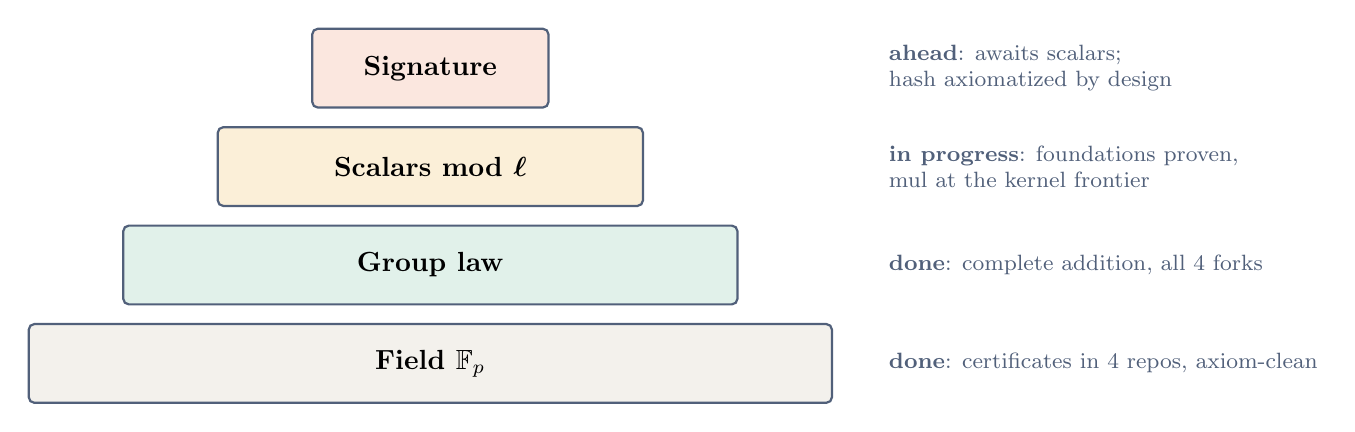
\begin{tikzpicture}[
  lay/.style={draw=ink2,thick,rounded corners=2pt,align=center,minimum height=1.0cm},
  st/.style={font=\footnotesize\color{ink2},anchor=west,align=left}
]
  \node[lay,fill=accentsoft,minimum width=3.0cm]  (sig) at (0,3.75) {\textbf{Signature}};
  \node[lay,fill=warnsoft,minimum width=5.4cm]    (sca) at (0,2.5)  {\textbf{Scalars mod $\boldsymbol{\ell}$}};
  \node[lay,fill=provensoft,minimum width=7.8cm]  (grp) at (0,1.25) {\textbf{Group law}};
  \node[lay,fill=codebg,minimum width=10.2cm]     (fld) at (0,0)    {\textbf{Field $\Fp$}};
  \node[st] at (5.7,0)    {\textbf{done}: certificates in 4 repos, axiom-clean};
  \node[st] at (5.7,1.25) {\textbf{done}: complete addition, all 4 forks};
  \node[st] at (5.7,2.5)  {\textbf{in progress}: foundations proven,\\ mul at the kernel frontier};
  \node[st] at (5.7,3.75) {\textbf{ahead}: awaits scalars;\\ hash axiomatized by design};
\end{tikzpicture}
\end{center}

\section{The group law: geometry becomes algebra}

An elliptic curve is a set of points $(x,y)$ satisfying an equation; for
Ed25519 it is the \emph{twisted Edwards} curve
$-x^2 + y^2 = 1 + d\,x^2 y^2$ over $\Fp$. The miracle: these points form a
\emph{group} under the addition law
\[
(x_1,y_1) + (x_2,y_2) \;=\;
\left(
\frac{x_1 y_2 + x_2 y_1}{1 + d\,x_1 x_2 y_1 y_2},\;
\frac{y_1 y_2 + x_1 x_2}{1 - d\,x_1 x_2 y_1 y_2}
\right).
\]
Two facts make this law a verifier's dream, and both carry Edwards-curve
signatures for exactly this reason. First, it is \textbf{complete}: for the
Ed25519 parameters those denominators are \emph{never zero} --- no special
cases for doubling, no branch for the identity, hence constant-time-friendly
code with no rarely-taken paths for bugs to hide in. (The proof, due to
Bernstein and Lange, is a jewel of quiet algebra: if a denominator vanished,
$d$ would have to be a square in $\Fp$ --- and it is not, which is a
\lean{decide}-scale fact away from primality.)

\begin{worked}{the completeness argument, derived to its hinge}
The Bernstein--Lange proof rewards a full pen-and-paper walk --- symbols,
not toy numbers, because the argument \emph{is} the real one at every
size. We run it on the Edwards curve $x^2 + y^2 = 1 + d x^2 y^2$ with
$d$ a non-square (Ed25519's twisted form adds decorations; the skeleton
is identical, and the exercises hand you the twist). Suppose, for
contradiction, points $(x_1,y_1)$, $(x_2,y_2)$ on the curve make a
denominator vanish: $\varepsilon := d\,x_1 x_2 y_1 y_2 \in \{\pm 1\}$.
A product equal to $\pm 1$ has no zero factor, so all four coordinates
are nonzero. Three moves, each checkable by expansion:

\emph{Move 1 --- square the assumption.} From $\varepsilon^2 = 1$:
$d^2 x_1^2 x_2^2 y_1^2 y_2^2 = 1$, which rearranges to
\[
1 \;=\; d x_1^2 y_1^2 \cdot d x_2^2 y_2^2 .
\]

\emph{Move 2 --- expand a well-chosen square.} Using
$x_1^2 + y_1^2 = 1 + d x_1^2 y_1^2$ (the curve, point 1) and
$\varepsilon x_1 y_1 = d x_1^2 y_1^2\, x_2 y_2$ (multiply the definition
of $\varepsilon$ by $x_1 y_1$):
\[
(x_1 + \varepsilon y_1)^2
= x_1^2 + y_1^2 + 2\varepsilon x_1 y_1
= 1 + d x_1^2 y_1^2 + 2\, d x_1^2 y_1^2\, x_2 y_2 .
\]

\emph{Move 3 --- substitute Move 1's $1$ and factor.} Replace the
leading $1$ by $d x_1^2 y_1^2 \cdot d x_2^2 y_2^2$ and pull out
$d x_1^2 y_1^2$:
\[
(x_1 + \varepsilon y_1)^2
= d x_1^2 y_1^2 \big( d x_2^2 y_2^2 + 1 + 2 x_2 y_2 \big)
= d x_1^2 y_1^2 \big( x_2^2 + y_2^2 + 2 x_2 y_2 \big)
= d\,\big(x_1 y_1 (x_2 + y_2)\big)^2 ,
\]
where the middle equality used the curve equation for point 2 backwards
($1 + d x_2^2 y_2^2 = x_2^2 + y_2^2$). Now the hinge: if
$x_2 + y_2 \neq 0$, divide ---
\[
d = \left( \frac{x_1 + \varepsilon y_1}{x_1 y_1 (x_2 + y_2)} \right)^{2},
\]
\textbf{$d$ is a square}. And if $x_2 + y_2 = 0$, rerun Moves 2--3 with
$(x_1 - \varepsilon y_1)^2$ to get $d \cdot (x_1 y_1 (x_2 - y_2))^2$
instead --- $x_2 - y_2$ cannot \emph{also} vanish (both would force
$x_2 = y_2 = 0$). Either way $d$ is a square in $\Fp$. But Ed25519's $d$
is \emph{not} --- one Legendre-symbol computation,
$d^{(p-1)/2} \equiv -1 \pmod p$, checkable by exactly the
square-and-multiply ladder of Chapter~\ref{ch:prime}, established once
as a constant fact in the verified development. Contradiction; no
denominator ever vanishes. Savor the architecture: one quadratic-residue
bit about one constant buys the \emph{total absence of special cases}
from every point addition ever executed --- and thereby the absence of
the rarely-taken branches where Chapter~\ref{ch:why}'s bugs live. That
is what ``a curve chosen for verifiability'' means in practice.
\end{worked} Second, the implementation
represents points \emph{projectively} (extended coordinates $(X:Y:Z:T)$,
avoiding division entirely) --- so the layer has its own denotation,
$(X:Y:Z:T) \mapsto (X/Z, Y/Z)$, and its own commuting squares built on the
field layer's specs. Same movie, one floor up: the verified group law in the
companion repos is precisely the statement that projective point addition
implements the rational formula above, all bounds included, for each fork's
own extraction.

\section{Scalars: a second field, and a frontier}

The group of curve points has order $8\ell$ with
$\ell = 2^{252} + 27742\ldots$ prime. Signature arithmetic happens in
exponents --- multiples of points --- so it is arithmetic mod $\ell$: a
\emph{second} finite field, with its own Rust implementation (radix-52
limbs, Montgomery multiplication) and its own denotation bridge. Nothing
conceptually new --- which is itself the lesson: the method \emph{scales
sideways} without new ideas.

\begin{worked}{sizing the group --- real constants, three-line audits}
The scalar layer's constants invite the same pen-and-paper audits as the
field's. The group order is $8\ell$ with
\[
\ell \;=\; 2^{252} + 27742317777372353535851937790883648493 ,
\]
that $38$-digit tail being an inseparable companion of anyone who works
on this layer. Three audits, each a few lines:

\emph{(1) Consistency with the curve.} A theorem of Hasse says an
elliptic curve over $\Fp$ has $p + 1 - t$ points with
$|t| \le 2\sqrt{p}$ --- so about $2^{255}$ points, within
$2^{128.5}$-ish. Check the claimed order:
$8\ell = 2^{3} \cdot 2^{252} + 8 \cdot (38\text{-digit}) =
2^{255} + (\text{a number} < 2^{129})$. Sits exactly in Hasse's window
around $p + 1 \approx 2^{255}$ ✓. The claimed structure is at least
arithmetically possible --- a thirty-second sanity check worth running on
\emph{any} curve parameter set someone hands you.

\emph{(2) The tail is not decoration.} Could a signature library
``round'' $\ell$ to $2^{252}$ --- who would notice? Anyone reducing a
$256$-bit hash output mod $\ell$: the reductions differ on roughly a
$2^{-124}$ slice of inputs (the interval lengths differ by the tail), and
the certified theorem \code{L\_val} in all four companion repos ---
\emph{the transpiled constant equals $\ell$, digit for digit} --- exists
precisely because ``a constant nobody can eyeball'' is where typos
retire. The proof is one \lean{decide}-scale comparison, and it has
teeth: change one digit of the Rust constant and \code{check-scalar.sh}
fails.

\emph{(3) Why the $8$s in the verification equation.} The full group has
order $8\ell = 2^3 \cdot \ell$, so (by the structure of finite abelian
groups) it decomposes as $\Z_8$-part $\times$ $\Z_\ell$-part: every point
splits as $X = T + Y$ with $T$ of order dividing $8$ (``torsion'') and
$Y$ of order dividing $\ell$. Multiply by $8$:
\[
8X \;=\; 8T + 8Y \;=\; \mathcal{O} + 8Y \;=\; 8Y
\]
--- the torsion component is annihilated, whoever chose it. An attacker
who tampers with a public key by adding a small-order point $T$ changes
$X$ but not $8X$; the cofactored equation $8sB = 8R + 8kA$ is therefore
immune to a whole class of malleability games that the uncofactored
$sB = R + kA$ is not. Three multiplications by $8$, bought by exactly the
three-line computation above.
\end{worked}

The engineering, however, has a frontier, and this book has told you enough
truth to locate it precisely. Scalar Montgomery multiplication mixes
$2^{256}$-scale coefficients into single certificate steps; this is the
kernel-capacity wall of Chapter~\ref{ch:field}, and it marks the current
working edge of the campaign: additions and the foundational constants are
certified (including the pleasing theorem that the code's constant
\code{L} \emph{is} $\ell$); the multiplication path is a construction site
with scaffolding --- decomposed lemmas, isolated carry steps ---
mid-assembly, honestly labeled in-repo.

\section{The apex: what ``verified signature'' will say}

EdDSA verification accepts $(R, s)$ on message $m$ under key $A$ iff
\[
8 s B \;=\; 8 R + 8\,H(R, A, m)\,A
\]
in the curve group ($B$ the base point, $H$ = SHA-512, the $8$s absorbing
the cofactor). The apex certificate will state: \emph{the extracted
verification routine returns true exactly when this equation holds} ---
given the two declared trusted-base entries you can already predict:
SHA-512 as an ideal hash (axiomatized by design --- hash function
correctness is a different mathematical universe), and the SIMD
point-multiplication backends (untranslatable, documented). Everything
between those declared boundaries and the field bedrock: kernel-checked,
axiom-clean, per fork.

Read that sentence again with Chapter~\ref{ch:honesty} eyes: it is a
\emph{smaller} claim than ``Ed25519 is verified!'' --- and that is exactly
why you can believe it.

\section{What you now know, and where to take it}

Take inventory. You can read a goal state and drive a proof; you know which
decision procedure owns which arithmetic fragment; you can build a
denotation bridge and state a two-clause spec; you can certify a prime with
a witness tree; you can audit anyone's certificate in one command and four
questions. That skill set is not Ed25519-specific --- it is the working
method of machine-checked mathematics applied to systems, and elliptic
curves were merely your first campaign.

Where to go from here, in increasing order of ambition:

\begin{itemize}[leftmargin=1.4em]
\item \textbf{Read a real proof end-to-end.} \code{FieldSpec.lean} in
  \code{dalek-ed25519-verified}, top to bottom, with this book as the
  decoder ring. Budget an afternoon; expect the odd hour of humility.
\item \textbf{Extend the pyramid.} The scalar layer's open lemmas are
  decomposed, labeled, and waiting; the repos' \code{CONTRIBUTING} notes
  state exactly what a finished brick looks like (spec shape, axiom
  audit, check-script entry). Frontier work, undergraduate-accessible.
\item \textbf{Verify something of yours.} Pick a 200-line pure function you
  actually use --- a parser, a checksum, a data structure --- write its
  denotation (what does it \emph{mean}?), state the square, prove it.
  The first solo bridge is the moment this stops being a course.
\item \textbf{Go deeper into the theory.} \emph{Theorem Proving in Lean 4}
  (the official text), \emph{Mathematics in Lean} (Mathlib's course), and
  the Lean Zulip --- an unusually welcoming expert community --- are the
  standard next doors.
\end{itemize}

\subsection*{Further reading, annotated}

\begin{itemize}[leftmargin=1.4em]
\item \emph{Theorem Proving in Lean 4} (Avigad, de Moura, et al.; free
online) --- the official text. Read it \emph{after} this book's
Chapters 2--5 and it will feel like meeting the extended family of
ideas you already know; its dependent-type chapters go far beyond our
needs and are worth the trip.
\item \emph{Mathematics in Lean} (the Mathlib community course) ---
hands-on Mathlib fluency: naming conventions, search strategies, the
algebra hierarchy. The fastest cure for ``I know the fact exists but
not its name,'' which will be your main bottleneck after this book.
\item \emph{The Lean Zulip} (\code{leanprover.zulipchat.com}) --- where
the community lives. Unusually welcoming to beginners; search before
asking, then ask well: a minimal example plus the goal state gets
expert answers in hours.
\item Bernstein \& Lange, \emph{Faster addition and doubling on
elliptic curves} (2007) --- the completeness proof this chapter's
worked example walked; readable with this book's preparation, and a
model of what ``designed for implementers'' mathematics looks like.
\item The RFC for EdDSA (RFC 8032) --- the signature scheme as
deployed, cofactor-$8$s and encoding details included. Read the
verification equation section against this chapter and notice how much
sharper your questions have become.
\item Project Everest / HACL$^{*}$ and Fiat Crypto --- the two other
major verified-crypto lineages (F$^{*}$-based and Coq-based
respectively), both shipping in real TLS stacks and browsers. Reading
their claims with your Chapter~\ref{ch:honesty} toolkit is instructive
in both directions: the methods differ, the honest-boundary discipline
rhymes.
\end{itemize}

\begin{aha}
One last reframe, the one this book was secretly about. ``Formal
verification'' sounds like bureaucracy --- forms, stamps, compliance. What
you actually practiced is closer to \emph{engineering's version of the
scientific method}: make the claim precise enough to be falsifiable, then
let an incorruptible referee try to falsify it, then publish the referee's
report with the assumptions itemized. Cryptography needed that discipline
first because its failures are silent and adversarial. It will not need it
last.
\end{aha}

\begin{tryit}
The graduation exercise. In the mini-system from
\code{exercises/Ch09.lean}, the file \code{exercises/Ch12.lean} plants a
\emph{deliberate off-by-one carry bug} in a variant \lean{add'} --- of
exactly the species from Chapter~\ref{ch:why}: correct on all limb pairs
except a thin boundary slice. Your final tasks: (1) write the spec ---
watch it \emph{refuse to prove}; (2) extract the counterexample from the
stuck goal state; (3) confirm by \lean{\#eval}; (4) fix the code and finish
the proof. That arc --- spec, refusal, counterexample, fix, certificate ---
is the entire profession in miniature. Welcome to it.
\end{tryit}

\section*{Exercises}

\exercise{(Paper) Verify Move 2 and Move 3 of the completeness worked
example by full expansion --- every term written out, nothing skipped.
Then adapt the argument's \emph{first} move to the twisted curve
$-x^2 + y^2 = 1 + d x^2 y^2$: where does the $-1$ enter, and why does the
argument want $-1$ to be a \emph{square} mod $p$? (Hint: $p = 2^{255}-19
\equiv 1 \pmod 4$, and for such primes $-1$ is a quadratic residue ---
which is not an accident of the curve designers.)}

\exercise{(Paper) In the group decomposition $X = T + Y$ (torsion of
order dividing $8$ plus a $\Z_\ell$ component), verify: (a) $8X = 8Y$;
(b) $8Y \neq \mathcal{O}$ whenever $Y \neq \mathcal{O}$ --- why does this
need $\gcd(8, \ell) = 1$, and where does the argument use that $\ell$ is
prime and $> 8$? (c) Conclude what an attacker who adds a small-order
point to a public key changes, and what they provably cannot change.}

\exercise{(Audit drill) Write down, from memory, the complete list of
what the apex certificate will \emph{assume} (its trusted base) and what
it will \emph{establish}, then check yourself against this chapter's
apex section. Anything you forgot is the thing to reread before you
audit a real system.}

\section*{Solutions and pathways}
\solutionsintro

\solhead{12.1}
\pathway For the expansion: Move 2 is the binomial square plus two
substitutions --- write $(x_1 + \varepsilon y_1)^2 = x_1^2 +
2\varepsilon x_1 y_1 + y_1^2$, then replace $x_1^2 + y_1^2$ via the curve
and $\varepsilon x_1 y_1$ via the definition. Move 3 is distributing
$d x_1^2 y_1^2$ and recognizing a perfect square. For the twist,
transport the curve equation and re-run Move 2.
\answer Move 2 fully expanded:
$(x_1+\varepsilon y_1)^2 = x_1^2 + 2\varepsilon x_1 y_1 + y_1^2$;
curve gives $x_1^2 + y_1^2 = 1 + dx_1^2y_1^2$; and
$\varepsilon x_1 y_1 = (d x_1 x_2 y_1 y_2)(x_1 y_1) = d x_1^2 y_1^2 x_2
y_2$ --- sum the three pieces to get the displayed line ✓. Move 3:
$d x_1^2 y_1^2 (d x_2^2 y_2^2 + 1 + 2 x_2 y_2)$; the curve for point 2
says $1 + d x_2^2 y_2^2 = x_2^2 + y_2^2$, so the bracket is
$x_2^2 + 2x_2y_2 + y_2^2 = (x_2+y_2)^2$, and
$d x_1^2 y_1^2 (x_2+y_2)^2 = d (x_1 y_1 (x_2+y_2))^2$ ✓. For the twisted
curve: $x_1^2 + y_1^2$ no longer appears --- the curve supplies
$y_1^2 - x_1^2$ --- so the well-chosen square must mix a factor
$\sqrt{-1}$ into the $x$'s (expand $(\sqrt{-1}\,x_1 + \varepsilon y_1)^2
= -x_1^2 + y_1^2 + 2\varepsilon\sqrt{-1}\,x_1 y_1$: the curve's
left-hand side appears exactly). That $\sqrt{-1}$ must \emph{exist} in
$\Fp$ for the argument to run --- hence the requirement that $-1$ be a
square, guaranteed by $p \equiv 1 \pmod 4$. The designers chose the
twist $a = -1$ \emph{because} it is a square mod this $p$: speed came
from the twist, completeness survived because of the residue class.
Parameters this well-matched are chosen, not lucky.

\solhead{12.2}
\pathway All three parts are order bookkeeping: $nZ = \mathcal{O}$
exactly when the order of $Z$ divides $n$.
\answer (a) $8X = 8T + 8Y$; the order of $T$ divides $8$, so
$8T = \mathcal{O}$, leaving $8Y$ ✓. (b) The order of $Y$ divides the
prime $\ell$, so it is $1$ or $\ell$. If $Y \neq \mathcal{O}$ the order
is $\ell$; then $8Y = \mathcal{O}$ would force $\ell \mid 8$ ---
impossible since $\ell > 8$ (it is $\approx 2^{252}$). This is where
both primality (order is $1$ or $\ell$, nothing between) and size come
in; $\gcd(8,\ell) = 1$ is the compact way to say ``multiplying by $8$ is
invertible on the $\Z_\ell$ part.'' (c) The attacker changes the point
$X$ (so: byte-level equality checks, hashes of the key, uniqueness
assumptions \emph{can} be affected --- real protocols have been bitten)
but provably cannot change $8X$, hence cannot affect the truth value of
any cofactored verification equation. The formal apex certificate
inherits exactly this robustness, and the ``$8$'' in its statement is
this exercise, immortalized.

\solhead{12.3}
\pathway Close the book. Write two columns: \emph{assumes} /
\emph{establishes}. Then open the apex section and diff.
\answer The list your memory should reproduce --- \emph{assumes}:
(1) SHA-512 behaves as an ideal hash (axiomatized by design, in the
trusted-base ledger); (2) the untranslatable SIMD point-multiplication
backends meet their stated specs (documented, per fork); (3) the three
standard Lean axioms; (4) the extraction pipeline preserves meaning
(one tool, pinned versions). \emph{Establishes}: for every input in the
bounds discipline, the extracted verification routine returns true
\emph{iff} $8sB = 8R + 8\,H(R,A,m)\,A$ in the curve group --- with
field arithmetic, group law, scalar arithmetic, and encoding each
carried by its own kernel-checked layer below. If your two columns
match this, you can audit a verification paper's abstract in ninety
seconds --- which was the promise on the book's cover, kept.

\begin{checkpoint}
The book's ending is a beginning, so the final checkpoint is prospective:
you should be able to (1) state what each pyramid layer claims and which
denotation it rides on; (2) explain to a security engineer why completeness
of the Edwards law matters to \emph{code}; (3) locate the current frontier
and say precisely why it is hard; and (4) name the next proof \emph{you}
intend to write. The authors of the companion repositories left the
scaffolding up on purpose.
\end{checkpoint}


\end{document}
